%%
%% Copyright 2022 OXFORD UNIVERSITY PRESS
%%
%% This file is part of the 'oup-authoring-template Bundle'.
%% ---------------------------------------------
%%
%% It may be distributed under the conditions of the LaTeX Project Public
%% License, either version 1.2 of this license or (at your option) any
%% later version.  The latest version of this license is in
%%    http://www.latex-project.org/lppl.txt
%% and version 1.2 or later is part of all distributions of LaTeX
%% version 1999/12/01 or later.
%%
%% The list of all files belonging to the 'oup-authoring-template Bundle' is
%% given in the file `manifest.txt'.
%%
%% Template article for OXFORD UNIVERSITY PRESS's document class `oup-authoring-template'
%% with bibliographic references
%%

%%%CONTEMPORARY%%%
\documentclass[unnumsec,webpdf,contemporary,large]{oup-authoring-template}%
%\documentclass[unnumsec,webpdf,contemporary,large,namedate]{oup-authoring-template}% uncomment this line for author year citations and comment the above
%\documentclass[unnumsec,webpdf,contemporary,medium]{oup-authoring-template}
%\documentclass[unnumsec,webpdf,contemporary,small]{oup-authoring-template}

%%%MODERN%%%
%\documentclass[unnumsec,webpdf,modern,large]{oup-authoring-template}
%\documentclass[unnumsec,webpdf,modern,large,namedate]{oup-authoring-template}% uncomment this line for author year citations and comment the above
%\documentclass[unnumsec,webpdf,modern,medium]{oup-authoring-template}
%\documentclass[unnumsec,webpdf,modern,small]{oup-authoring-template}

%%%TRADITIONAL%%%
%\documentclass[unnumsec,webpdf,traditional,large]{oup-authoring-template}
%\documentclass[unnumsec,webpdf,traditional,large,namedate]{oup-authoring-template}% uncomment this line for author year citations and comment the above
%\documentclass[unnumsec,namedate,webpdf,traditional,medium]{oup-authoring-template}
%\documentclass[namedate,webpdf,traditional,small]{oup-authoring-template}

\onecolumn % for one column layouts

%\usepackage{showframe}

\graphicspath{{Fig/}}

% line numbers
%\usepackage[mathlines, switch]{lineno}
%\usepackage[right]{lineno}

\theoremstyle{thmstyleone}%
\newtheorem{theorem}{Theorem}%  meant for continuous numbers
%%\newtheorem{theorem}{Theorem}[section]% meant for sectionwise numbers
%% optional argument [theorem] produces theorem numbering sequence instead of independent numbers for Proposition
\newtheorem{proposition}[theorem]{Proposition}%
%%\newtheorem{proposition}{Proposition}% to get separate numbers for theorem and proposition etc.
\theoremstyle{thmstyletwo}%
\newtheorem{example}{Example}%
\newtheorem{remark}{Remark}%
\theoremstyle{thmstylethree}%
\newtheorem{definition}{Definition}

% \newcommand{\hlc}[2][yellow]{{%
%     \colorlet{foo}{#1}%
%     \sethlcolor{foo}\hl{#2}}%
% }

\tikzset{fit margins/.style={/tikz/afit/.cd,#1,
    /tikz/.cd,
    inner xsep=\pgfkeysvalueof{/tikz/afit/left}+\pgfkeysvalueof{/tikz/afit/right},
    inner ysep=\pgfkeysvalueof{/tikz/afit/top}+\pgfkeysvalueof{/tikz/afit/bottom},
    xshift=-\pgfkeysvalueof{/tikz/afit/left}+\pgfkeysvalueof{/tikz/afit/right},
    yshift=-\pgfkeysvalueof{/tikz/afit/bottom}+\pgfkeysvalueof{/tikz/afit/top}},
    afit/.cd,left/.initial=2pt,right/.initial=2pt,bottom/.initial=2pt,top/.initial=2pt}

\begin{document}

\journaltitle{submitted to Journal of Cybersecurity}
\DOI{DOI HERE}
\copyrightyear{Aug 30th, 2022}
\pubyear{Aug 30th, 2022}
\access{Advance Access Publication Date: Day Month Year}
\appnotes{Paper}

\firstpage{1}

%\subtitle{Subject Section}

\title[Collective Action in Cybersecurity]{Efficient Collective Action for Tackling Time-Critical Cybersecurity Threats}

\author[1,2,$\ast$]{S\'ebastien Gillard \ORCID{0000-0002-3237-8599}}
\author[1,3,4]{Dimitri Percia David \ORCID{0000-0002-9393-1490}}
\author[3]{Alain Mermoud \ORCID{0000-0001-6471-772X}}
\author[1,5]{Thomas Maillart \ORCID{0000-0002-5747-9927}}

\authormark{S.Gillard et al.}

\address[1]{Information Science Institute, Geneva School of Economics and Management, University of Geneva}
\address[2]{Department of Defense Economics, Military Academy at ETH Zurich}
\address[3]{Cyber-Defence Campus, armasuisse Science and Technology}
\address[4]{Institute of Entrepreneurship \& Management, School of Management, University of Applied Sciences of Western Switzerland (HES-SO Valais-Wallis)}
\address[5]{Citizen Cyber Lab, University of Geneva}


\corresp[$\ast$]{Corresponding author: Sébastien Gillard, Kaserne Reppischtal, CH-8903 Birmensdorf. E-mail: \href{mailto:sebastien.gillard@etu.unige.ch}{sebastien.gillard@etu.unige.ch}}

\received{Date}{0}{Year}
\revised{Date}{0}{Year}
\accepted{Date}{0}{Year}

%\editor{Associate Editor: Name}

%\abstract{
%\textbf{Motivation:} .\\
%\textbf{Results:} .\\
%\textbf{Availability:} .\\
%\textbf{Contact:} \href{name@email.com}{name@email.com}\\
%\textbf{Supplementary information:} Supplementary data are available at \textit{Journal Name}
%online.}

\abstract{The latency reduction between the discovery of vulnerabilities, the build-up and dissemination of cyber-attacks has put significant pressure on cybersecurity professionals. For that, security researchers have increasingly resorted to collective action in order to reduce the time needed to  characterize and tame outstanding threats. Here, we investigate how joining and contributions dynamics on MISP, an open source threat intelligence sharing platform, influence the time needed to collectively complete threat descriptions. We find that  performance, defined as the capacity to characterize quickly a threat event, is influenced by (i) its own complexity (negatively), by (ii) collective action (positively), and by (iii) learning, information integration and modularity (positively). Our results inform on how collective action can be organized at scale and in a modular way to overcome a large number of time-critical tasks, such as cybersecurity threats.}
\keywords{cybersecurity; information sharing; collective action; information integration; economies of scales; Malware Information Sharing Platform (MISP).}

% \boxedtext{
% \begin{itemize}
% \item Key boxed text here.
% \item Key boxed text here.
% \item Key boxed text here.
% \end{itemize}}

\maketitle

\section{Introduction}
\label{sec1}

From Computer Emergency Readiness Teams (CERT) established in the nineties \cite{sridhar_cybersecurity_2021}, to information-sharing analysis centers (ISACs) \cite{gal-or_economic_2005}, to bug bounty programs \cite{maillart_given_2017, sridhar_hacking_2021}, collective action has long been used and recognized as key for the gathering, the integration and the sharing of critical cybersecurity information \cite{bohme_back_2016,laube_strategic_2017}. The reason for resorting to information-sharing as a form of collective action stems from the complexity associated with the continuous and somewhat decentralized (e.g., open source software) adaptation of hardware and software in information systems \cite{brady_murphys_1999, stojkovski_whats_2021}. Although the Internet has largely developed through an open source spirit \cite{levy_hackers_2010, benkler_penguin_2011, benkler_wealth_2006} with significant positive externalities \cite{katz_network_1985, shapiro_information_1999}, information-sharing has remained difficult when it comes to cybersecurity \cite{laube_strategic_2017}. The expansion of threats in volume, severity and span has further challenged information infrastructures. Hence, it has forced further cooperation through information-sharing  \cite{wagner_misp_2016}. While their utility has been somewhat confirmed by their wide adoption, there is a dearth of knowledge regarding how these collective action platforms concretely bring performance when addressing cybersecurity threats. For instance, cybersecurity has become increasingly time-critical and demands ever faster reaction time. Determining the chances that a threat will be fully characterized on time for security officers to act upon before attacks actually start has become crucial \cite{zibak_cyber_2019}.

Here, we investigate $39\,639$ threat events contributed by 485 organizations to a MISP\footnote{MISP stands for ``Malware Information Sharing Platform."}  information-sharing platform \cite{wagner_misp_2016} operated by the Computer Incident Response Center Luxembourg (CIRCL). We specifically study how collective action unravels through information integration and how it brings significant economies of scale in terms of time needed to fully characterize cybersecurity threats (i.e., performance). We resort to a multivariate cross-sectional regression with ordinary least squares method, and we find that (i) the number of organizations engaged in information-sharing, (ii) their acquired experience in the events completion, (iii) the proportion of information integration and (iv) modularity increase performance.

The remainder of this article is organized as follows. The \textbf{\hyperref[sec:background]{Background}} section covers the literature from the perspectives of social dilemma, productivity and information integration in collective action in general and for cybersecurity. The \textbf{\hyperref[sec:data]{Data}} section introduces MISP and presents the data. We then introduce the \textbf{\hyperref[sec:theory]{Theoretical Framework}} followed by the research \textbf{\hyperref[sec:hypotheses]{Hypotheses}} section and the \textbf{\hyperref[sec:method]{Method}}. We then present the \textbf{\hyperref[sec:results]{Results}} and provide a \textbf{\hyperref[sec:discussion]{Discussion}} section before \textbf{\hyperref[sec:conclusion]{Concluding}}.

\section{Background}
\label{sec:background}
Knowledge sharing in cybersecurity has been considered as a crucial way to overcome number of vulnerabilities \cite{mell_common_2006} and threats \cite{sridhar_cybersecurity_2021}. It is however bound to limiting factors on the one hand, such as social dilemma, as well as enhancing return-on-scale effects on the other hand. Here, we review the literature on (i) social dilemma and productivity of collective action, and on (ii) challenges associated with information integration. We then review the state-of-the-art research in (iii) information sharing for cybersecurity.

\subsection{Social Dilemma and Productivity in Collective Action}
\label{social_dilemma}

According to Olson's logic of collective action, small communities are more able to provide collective goods \cite{olson_logic_1971}. The central argument is that minor interests will be over-represented and diffuse majority interests trumped, due to a free-rider problem \cite{anesi_moral_2009,varian2004system}. This free-riding effect is stronger for larger groups \cite{esteban_collective_2001}. For instance, while Dejean et al. \cite{dejean_olsons_2010} found a positive relation between the size of a community and the amount of collective good provided, they paradoxically also found a decreased propensity by individuals to cooperate as the size of the community increases. Beyond the increase of the community, due to the selfish behavior of the community members, the community efficiency to produce public goods depreciates \cite{KOUTSOUPIAS200965}.
Yet, there is overwhelming evidence that large crowds can be organized in order to establish successful online collective action. Examples include peer-to-peer networks \cite{asvanund_empirical_2004, dejean_olsons_2010},  Wikipedia \cite{klein_virtuous_2015},  Stack Overflow \cite{wang_empirical_2013}, communities of open source software developers \cite{hippel_open_2003,sornette2014much}. %Gächter et al.\cite{gachter_initiating_2010} found that social dilemma is more critical at the onset of a project and thus, knowledge sharing is more fragile early on. 
The Dejean et al. paradox may at least partially resolved by considering that (i) the distribution of effort is highly skewed, with few contributors providing most effort, and (ii) the dynamics of contribution are highly non-linear \cite{sornette2014much,maillart_aristotle_2019,muric_collaboration_2019}. Taken together, these phenomena are associated with positive return-on-scale of production \cite{sornette2014much}, which may be hindered by coordination costs \cite{scholtes_aristotle_2016}. Super-linear productivity has been debated at length in organization and management sciences. Investigations of how the number of members, temporal dynamics of events generated can influence positively outputs in way that is greater than the sum of the outputs related to each element of the system (i.e., exhibiting super-linear growth patterns). Research has successfully delivered hints to improve the performance of organization \cite{tziner_effects_1985, sundstrom_work_1990, cohen_what_1997, neuman_team_1999} by fine-tuning complementary mechanisms within the organization \cite{ennen_whole_2010}, which also foster innovation \cite{sacramento_team_2006}.

\subsection{Information Integration and Modularity}
\label{sec:knowledge_integration}

One key aspect of generating return-on-scale in knowledge production is information integration. The management of information resources has become central to organizations \cite{nonaka_dynamic_1994}, so that knowledge appears as an utmost strategic resource \cite{grant_prospering_1996}. For instance, there is growing evidence in science that greater teams create more impacting knowledge \cite{wuchty_increasing_2007}. If knowledge is so important, the fundamental capability of an organization has to be considered as the specialized knowledge of each organization member. Its integration shall provide a competitive advantage \cite{grant_prospering_1996,lawrence_differentiation_1967}. With the emergence of virtual exchanges, firms are increasingly seen as distributed knowledge systems \cite{majchrzak_catalyst_2018}. Yet, new interaction methods present various new constraints in term of mutual understanding, contextual knowledge or techniques (e.g., memory, connectivity), which lead to asymmetries in information integration.

%Alongside this dominant theory, other ideas appear to be promising based when considering collective intelligence in groups \cite{woolley_evidence_2010}.
In this respect, the tremendous development of online collaboration platforms, as tools for governance strategy and knowledge management, highlights the importance of information-sharing \cite{safa_information_2016}. These platforms promote knowledge transfer by generating modular collaborative units \cite{mockus_case_2000}. One may consider that individuals, or groups of individuals, composing a subsystem (i) bring added value in their own specific field (differentiation), in order to (ii) produce a complex good by pooling together this added value (integration). Following Arrow \& Debreu \cite{kenneth_j_arrow_and_gerard_debreu_existence_1954}, differentiation and integration have been a focal point in optimizing the structure of organizations \cite{ravasi_organising_2001, huang_knowledge_2003}. In fact, differentiation considers segments of a system into subsystems. Each subsystem develops a part of a task, while the integration focuses on the interactions between these subsystems in order to accomplish the entire task \cite{lawrence_differentiation_1967,engel_integrated_2018}. Recently, Engel and Malone used the theory of consciousness as information integration \cite{tononi_consciousness_1998} to measure information integration computer systems and on collaborative platforms \cite{engel_integrated_2018}.

\subsection{Collective Action and Information Integration for Cybersecurity}

As early as twenty years ago, the first Computer Emergency Readiness Teams (CERT) and Information Sharing and Analysis Centers (ISACs) have been established as a central resource for sharing information on cybersecurity threats to critical infrastructures \cite{zheng_cyber_2015}. Nowadays, threat intelligence platforms help organizations aggregate, correlate, and analyze threat data from multiple sources in (almost) real-time to support defensive actions \cite{he_perspectives_2018}. Further, open source solutions have been proposed as a counterweight to cyber-criminals successfully working together \cite{bohme_back_2016}.
The swift evolution of cyber-threats has forced organizations and governments to develop new strategies \cite{meier_feedrank_2018} in order to reduce the risks of security breaches \cite{safa_information_2016}. Although information sharing
is an interesting way to enhance cybersecurity, it is believed to be thwarted by social dilemma. Without trust, commitment and shared vision between stakeholders, organizations are reluctant to share information due to the fear of disclosure, reputation risk or loss of competitive power \cite{mermoud_share_2019}. As such, information-sharing can be considered as a marketplace on which transactions occur and knowledge is transferred \cite{perciadavid_knowledge_2020}. However, human beings have a tendency to not optimize organizational goals \cite{mermoud_governance_2019} in the absence of selective incentives \cite{oliver_reward_1980} and – in the case of collective action – might adopt a selfish behavior that are not conducive to the overall goal of sharing information \cite{laube_strategic_2017}. As a consequence, cybersecurity professionals share probably less information than desirable, leading to a knowledge asymmetry to the advantage of the attackers \cite{laube_strategic_2017}. In particular, stakeholders strategically select their contributions to share (i.e., quantity and quality), leading to truncated and imperfect information sharing. However, when the situation is extraordinarily difficult, the behaviors tends to become unselfish, leading to an increase of the contributions \cite{hirshleifer_weakest-link_1983}.
In this context, specially crafted forms of cybersecurity information-sharing platforms have developed, such as bug bounty marketplaces. These platforms act as a trusted third-party between security researchers and software editors \cite{maillart_given_2017}. Further, in cybersecurity, resource belief, usefulness belief, and reciprocity belief are all positively associated with knowledge absorption, whereas reward belief is not \cite{perciadavid_knowledge_2020}. These empirical results show that functional cybersecurity information-sharing indeed requires to overcome social dilemma and goes beyond simple reward expectations, but foremost requires that information-sharing is efficient in a context that increasingly requires to address time-critical threats.

\section{Data}
\label{sec:data}

To understand the nuts and bolts of cybersecurity information-sharing, we resort to {\it MISP Project},\footnote{\url{https://www.misp-project.org/}} a popular open source platform, which is used e.g., by the North Atlantic Treaty Organization (NATO).\footnote{\url{https://misp.ncirc.nato.int}} MISP stands for {\it Malware Information Sharing Platform and Threat Sharing}. Although it carries the word malware in its name, MISP is a threat intelligence platform on which people can share, store and collaborate on all sorts of incidents (e.g., COVID-19 MISP community,\footnote{\url{https://covid-19.iglocska.eu}} but primarily cybersecurity threats. These threats (i.e., events) are characterized by indicators of compromise (i.e., attributes), which are contributed by a multitude of organizations. Appendix \ref{Appendix:MISP_description} provide a detailed description of MISP. 

There are advantages in using MISP as an object of research. First, it is an open source software. This allows to understand in much detail how the platform is designed and works. Second, a number of threat information sharing communities use MISP to share relatively openly their threat intelligence. Here, we use the whole history of a MISP instance maintained by the Computer Incident Response Center Luxembourg (MISP CIRCL), i.e., the Luxembourg CERT.

As of 8 February 2022, the MISP CIRCL instance is a community of $1\,908$ organizations (respectively $4\,013$ users), which have contributed $39\,639$ events, $9\,099\,685$ attributes and $3\,786$ tags since 10 November 2008. Table \ref{tab:top_10_contributors} shows the ten most involved organizations. One can see that the number of events contributed by organizations is highly skewed. Indeed, Figure \ref{fig:org}A shows that the complementary cumulative distribution function exhibits a power law $P(X_{E}>x_{E}) \sim 1/x_{E}^{\mu_{E}}$ with $\mu_{e} = 0.54(4)$ (c.f., Appendix \ref{sec:ExploA} for details on the fitting method). One may additionally note that $1,423$, i.e., around $75\%$, of organizations do not participate in sharing threat information as a collective good with the broad MISP CIRCL community. These organizations may however consume information or share threat information privately within informal sub-groups, which cannot be observed. Similarly to $P(X_E > x_{E})$, the distributions of attributes $P(X_{A} > x_{A})$ and tags $P(X_{T} > x_{T})$ per event, depicted in Figure \ref{fig:CCDFs}, follow power laws with exponents respectively $\mu_A = 0.64(1)$ (with an upper cut-off around $A_{upper} = 10^5$) and $\mu_{T} = 2.26(6)$. It is additionally important to consider that only $22\,423$ (i.e., around $57\%$) events have been marked as completed (see Appendix \ref{Appendix:MISP_description} for the justification), suggesting that either threat analysis is complicated or that users tend to forget to formally close a large number of events. The cumulative number of tags $N_{T,\textrm{cum}} = 116\,407$ used is bigger than the unique tags amount $N_{T_U} = 3\,786$. Thus, there is a massive reuse of already existing tags.
    
We further observe that organizations have joined MISP CIRCL following an almost perfect linear relation $N_O(t) \sim \alpha_O \cdot t $ with $\alpha_O = 0.79(1)$ ($R^2 = 0.99$ and $p<10^{-2}$) with $161$ organizations initially joining MISP CIRCL instance on 14 September 2015, the presumed date of official start. Figure \ref{fig:org}B, not only shows the almost linear organization joining rate, but also how many events each organization has contributed over time. One see that the contribution effort is highly heterogeneous. It is also worth noting that event contributions started on 10 November 2008, long before the first organizations joined MISP CIRCL instance. This can be explained in the following way: organizations run first their MISP instance locally. At some point, they join the MISP CIRCL community and share at once all their non-private threat intelligence, yet with the nominal event timestamp, which may well be in the past. Also, it is likely that the linear organization joining function may be the result of a highly vetted joining process, controlled by CIRCL.

    \begin{figure}[ht]
    \centering
    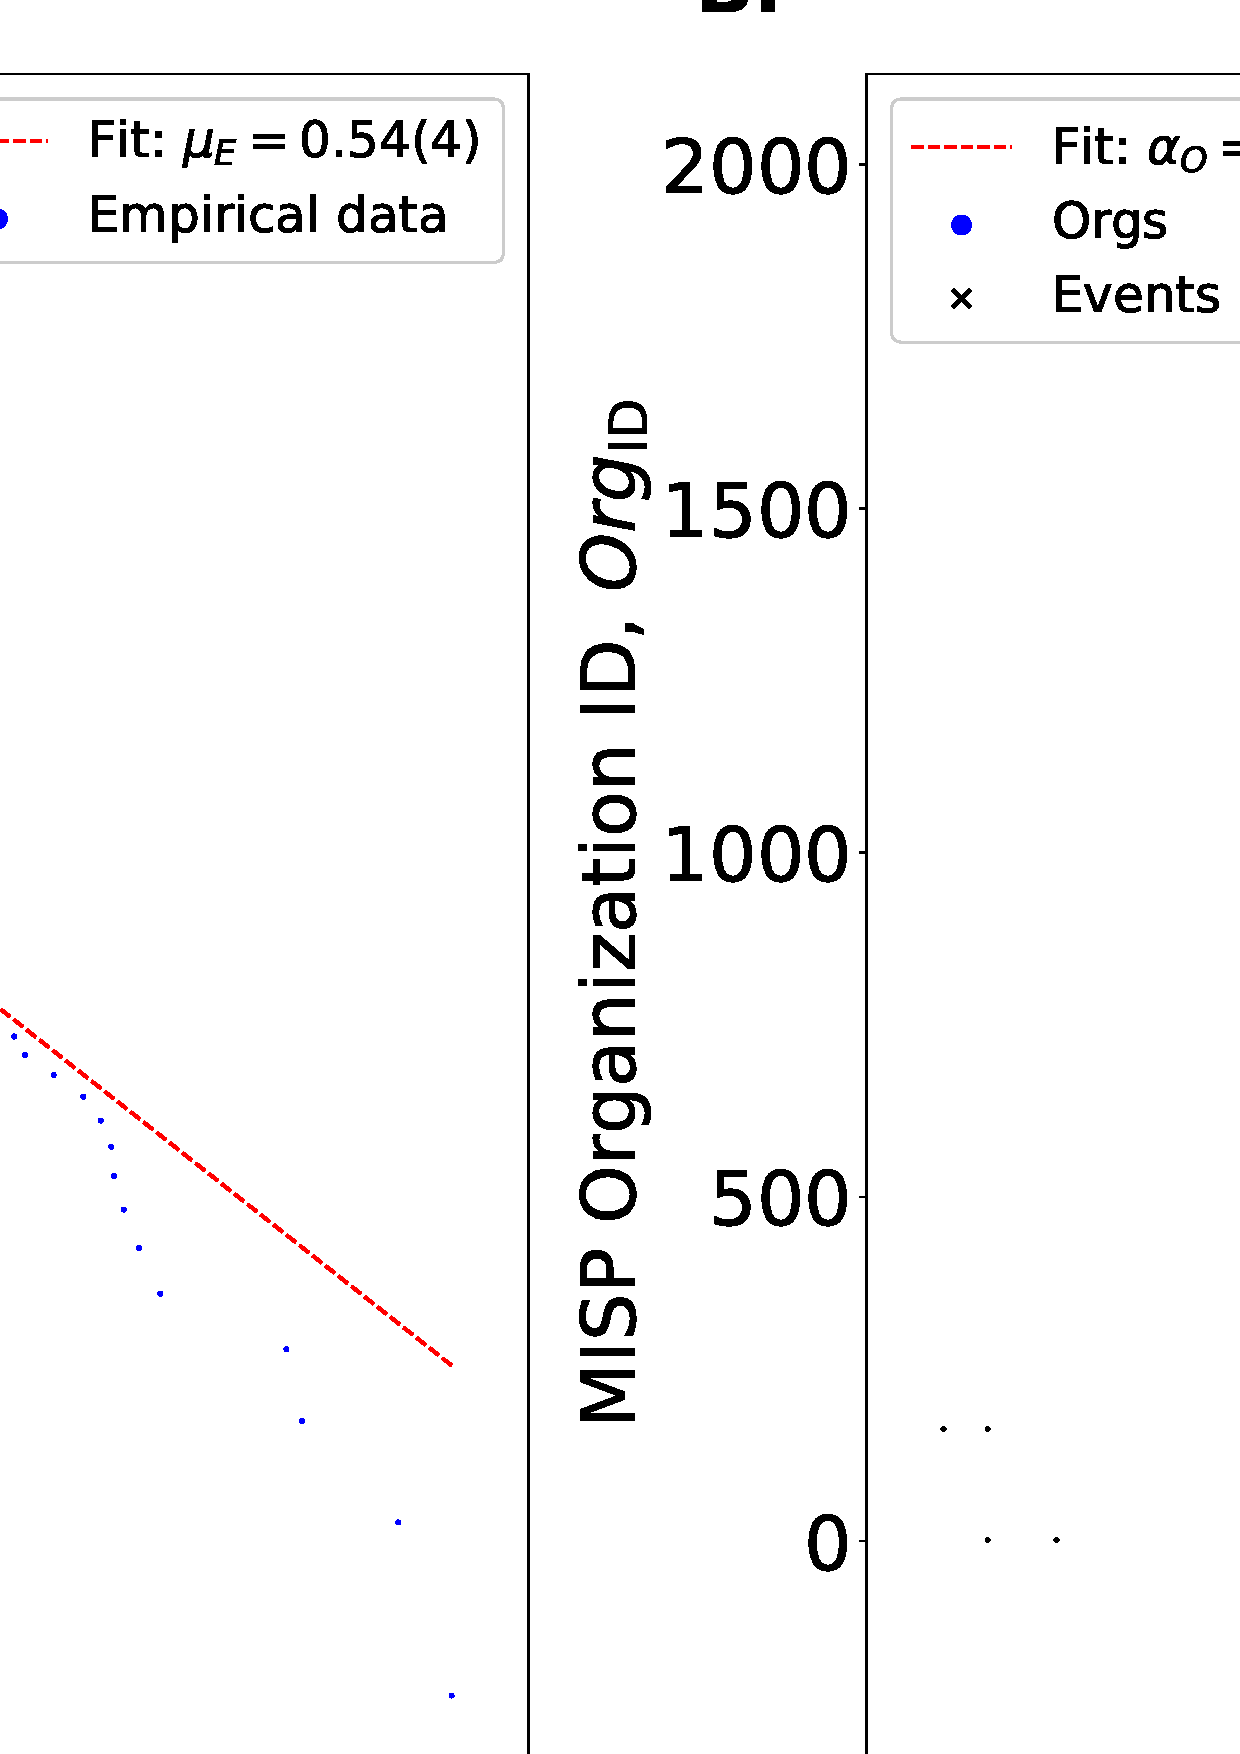
\includegraphics[width=\textwidth]{Figure1.png}
    \caption{{\bf A.} Complementary cumulative distribution function (CCDF) of events per contributing organization, which is best described by a power law distribution $P(X_E>x_E) \sim 1/{x_E}^{\mu_E}$ with $\mu_E = 0.54(4)$. The fit and the goodness-of-fit, provided by the Kolmogorov-Smirnov statistics test, are obtained with the \texttt{Python} library \texttt{plfit}. {\bf B.} Curve of the joining organizations (in blue) has followed, after the September 14, 2015, the presumed date of official start, a linear growth with slope $\alpha_O = 0.79(1)$, ($R^2 = 0.99,~p\textrm{-value} < 10^{-2}$). The events contributed by the organizations have been added (in dark gray), the distribution shows the heterogeneity of organizations efforts.} 
    \label{fig:org}
    \end{figure} 
    \begin{figure}[ht]
    \centering
    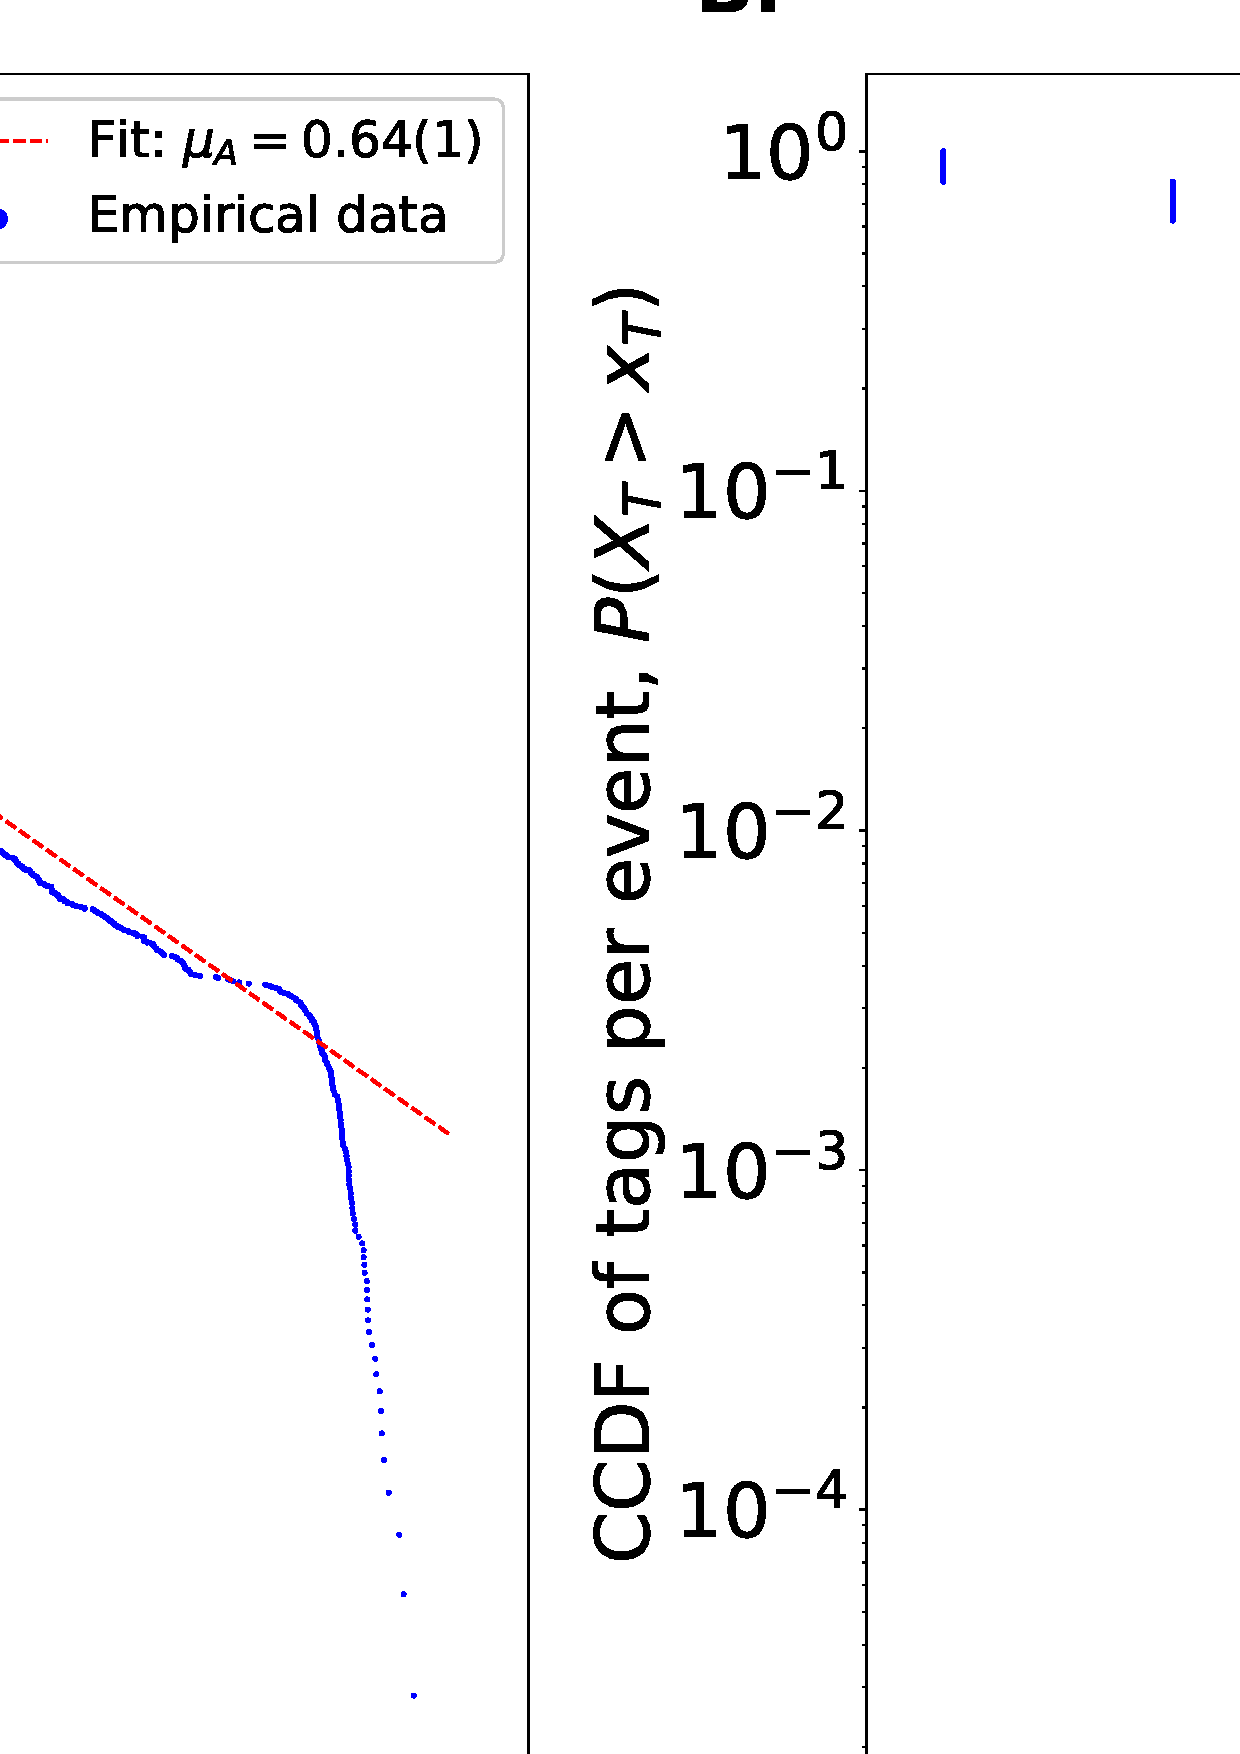
\includegraphics[width=\textwidth]{Figure2.png}
    \caption{{\bf A.} Complementary cumulative distribution function (CCDF) of attributes encapsulated in an event, which is best described by a power law distribution $P(X_A>x_A) \sim 1/{x_A}^{\mu_A}$ with $\mu_A = 0.64(1)$. {\bf B.} CCDF of tags attached to an event which is best described by a power law distribution $P(X_T > x_T) \sim 1/x_T^{\mu_T}$ with $\mu_T = 2.26(6)$. The fits and the goodness-of-fits, provided by the Kolmogorov-Smirnov statistics test, of panels A and B are obtained with the \texttt{Python} library \texttt{plfit}.}
    \label{fig:CCDFs}
    \end{figure}
    
\subsection[Reduction of the Completion Time of Events \texorpdfstring{$\Delta t_C$}{\textDelta}]
  {Reduction of the Completion Time of Events $\Delta t_C$}



Following the method described in the Appendix \ref{sec:ExploA}, we can treat the data and, from them, generate the Figure \ref{fig:Deltat}B. As explained in the appendix, by playing with the axis, we remark that when the axes are in linear-logarithmic scale, the data depict two straight lines. From this observation, we can deduce that $\Delta t_C(t)$ follows an exponential decrease in phase. By applying a binning by month and computing the mean value $\overline{\Delta t_C}$ for each bin, we see a first phase that extends from 2011 to $\Gamma$ (i.e., the transition between the two phases at the end of 2019) which decrease slower than the second phase from $\Gamma$ to today. By applying the linear regression on the data, according to the equation $\eqref{eq:lin-log}$, we confirm that $\Delta t_C$ exhibits an exponential decrease:
    \begin{align}
        \Delta t_C(t) =
        \begin{cases}
        \sim 10^{\beta_{\Delta}^1 \cdot t}, \textrm{ for } t \in [2011,\Gamma[, \\
        \sim 10^{\beta_{\Delta}^2 \cdot t}, \textrm{ for } t \in [\Gamma,2022],
        \end{cases}
    \end{align}
    \noindent
    where
    \begin{quote}
        \begin{itemize}
            \item[--] $\beta_{\Delta}^1 = (- 6.32 \pm 0.91) \times 10^{-3}$ is the exponential decrease of the first part regression and
            \item[--] $\beta_{\Delta}^2 = (-7.12 \pm 0.59) \times 10^{2}$ is the exponential decrease of the second part regression.
        \end{itemize}
    \end{quote}

The fit from the linear is of high quality since its Pearson's determination coefficient $R^2 =0.86$ and its $p\textrm{-value}< 10^{-2}$.
Hence, the time $\Delta t_C$ to complete an event decreases over time, indicating an improvement of performances of the MISP CIRCL instance.

\begin{figure}[ht]
\centering
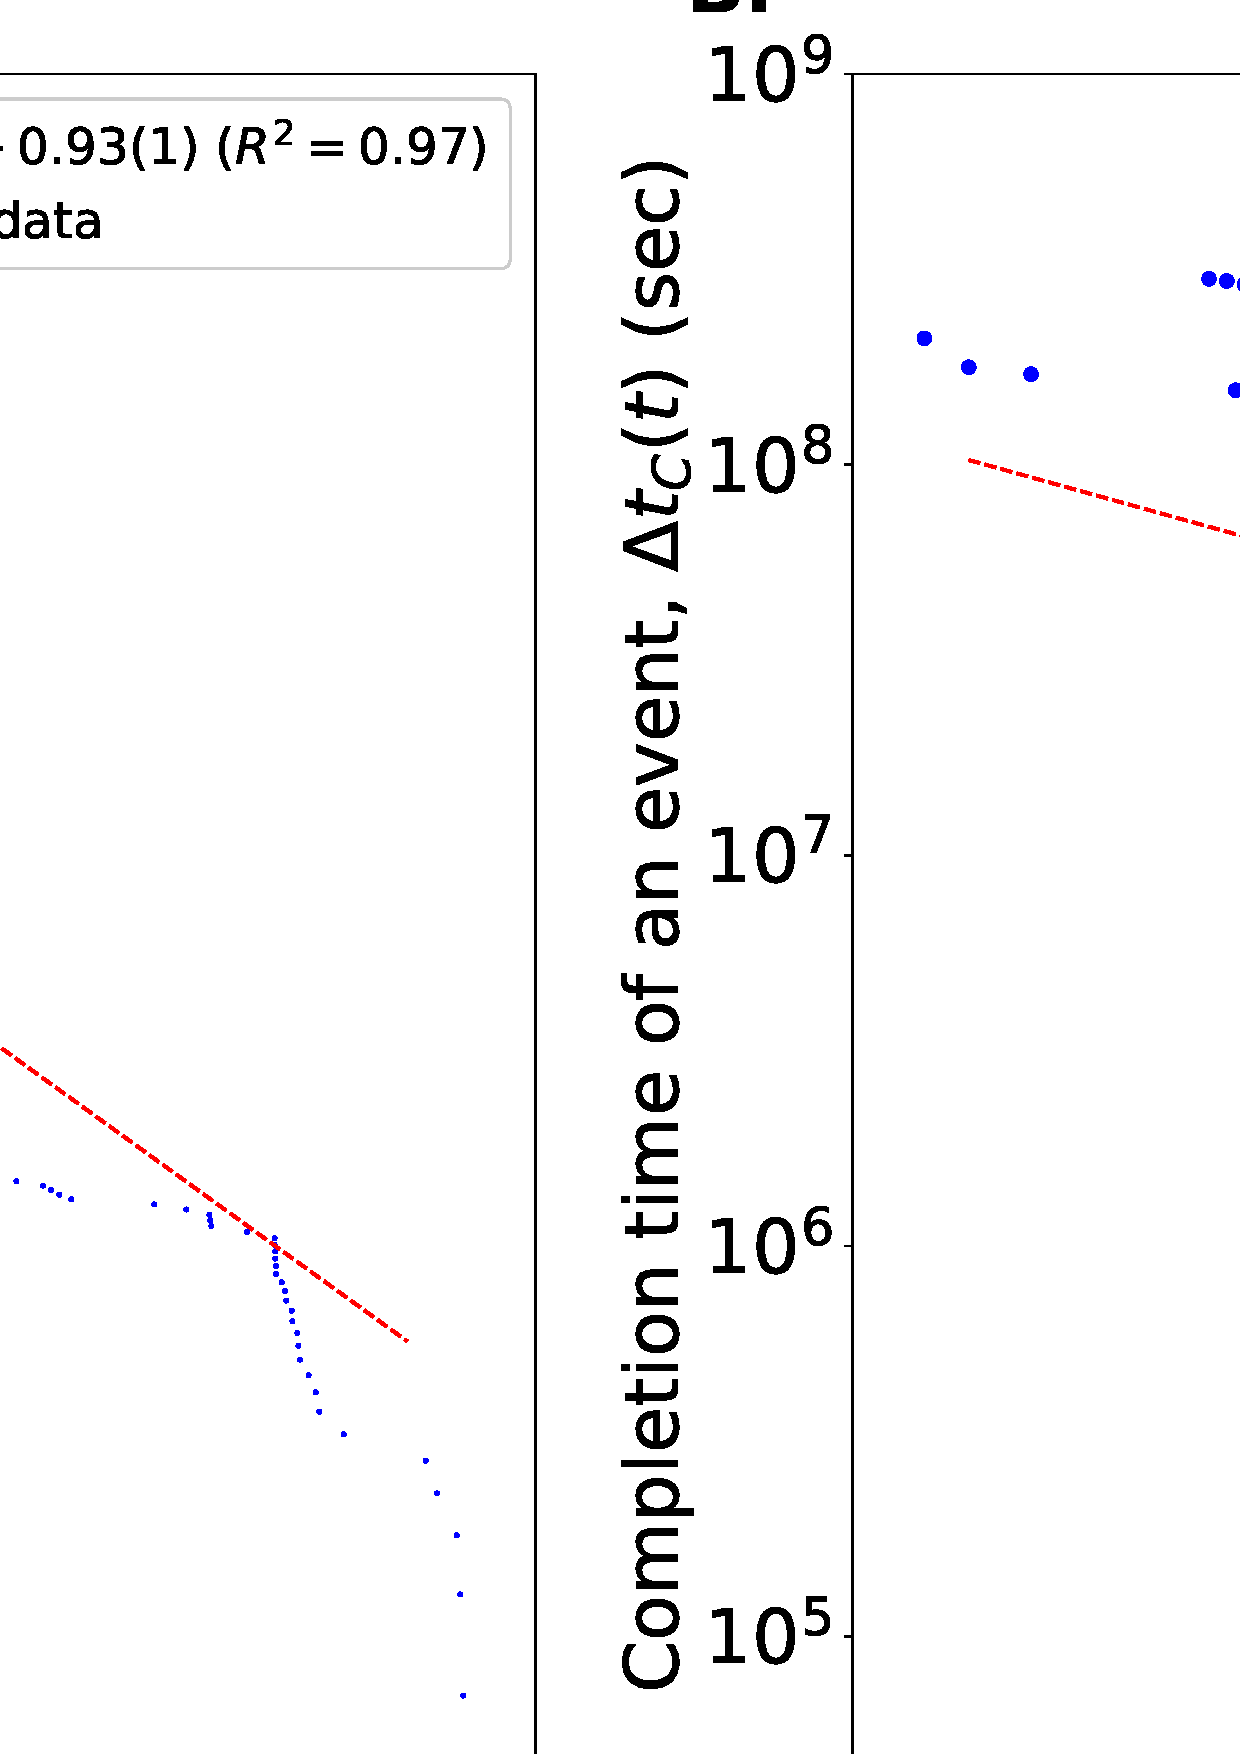
\includegraphics[width=\textwidth]{Figure3.png}
\caption{{\bf A.} Complementary cumulative distribution function (CCDF) of the completion time $\Delta t_C$, which is best described by a decreasing exponential distribution $P(X_{\Delta} < x_{\Delta}) \sim 10^{\beta_{\Delta}}$ with $\beta_{\Delta} = -0.93(1)$. {\bf B.} Completion time $\Delta t_C$ of events over the time. The data (blue dots) represents the mean value of $\Delta t_C$ binned monthly. The data depict an exponential decrease in two phases, changing at $\Gamma$ (green dotted line), fitted by linear regression (dashed red line), $\Delta t_C(t) \sim (-6.32 \pm 0.91) \times 10^{-2}$ for $t \in [2011,\Gamma[$ and $\Delta t_C(t) \sim (-7.12 \pm 0.59) \times 10^{-2}$ for $t \in [\Gamma,2022]$ ($R^2 = 0.86,~p\textrm{-value} < 10^{-2}$). The fits and their goodness-of-fits, provided by the Pearson's coefficient of determination $R^2$ and the $p$-value for the Wald test, of panels A and B are obtained with the \texttt{Python} library \texttt{scipy.stats.linregress}.}
\label{fig:Deltat}
\end{figure} 

\section{Theoretical Framework}
\label{sec:theory}
Collective action is thought to be a fundamental tool to overcome sprawling and increasing time-critical cybersecurity threats \cite{mermoud_three_2019,bouwman_governance_2018,wagner_cyber_2019}. Yet, despite numerous studies of online platforms fostering collective action \cite{bouwman_helping_2022,mccoll_performance_2014}, very little evidence has been uncovered linking the organisation of collective action with group performance as an output. By investigating the MISP threat management platform run by the Computer Incident Response Center Luxembourg (CIRCL), we have a unique chance to better understand how collective action is organized to tackle time-critical cybersecurity threats.

We posit that the  performance of collective platforms devoted to the resolution of time-critical tasks at scale, such as MISP, pull from progressively building a knowledge and action environment, made of organizations, which contribute to the resolution of events and, at the same time, bring returns of scale through (i) gaining own experience and (ii) sharing and integrating knowledge, which is associated with increased performance. We further posit that, in order to offset decreasing return-of-scale due to increased groups size and coordination costs \cite{scholtes_aristotle_2016}, the organization of collective action must adapt in a modular way \cite{baldwin_architecture_2006}, as it has already been witnessed in several open source projects \cite{narduzzo_role_2005,langlois_hackers_2008}.

We test our theory of {\it collective action for tackling time-critical tasks}, through a set of three hypotheses and six sub-hypotheses to understand how time completion performance is achieved for events, given (i) the nature of event, (ii) the collective action environment and (iii) the knowledge integration environment at the time of event arrival (c.f., ``\hyperref[sec:hypotheses]{Hypotheses}" section). We proceed with an exploratory approach to test our theory by resorting to a multivariate cross-sectional regression with ordinary least squares method (c.f., ``\hyperref[sec:method]{Method}" and ``\hyperref[sec:results]{Results}" sections).

\section{Hypotheses}
\label{sec:hypotheses}

To explain how event completion time has evolved, we consider their {\it intrinsic nature}, i.e., number of attributes and tags required to characterize events. We then define {\it event complexity}, the {\it overall collective action environment} and how {\it knowledge is integrated}. We hypothesize that these three factors significantly influence collective action performance, in terms of improved completion time in characterizing threat events.


\subsection{Event Complexity Hinders Performance (H1)}

First, events are not all equal: while some are fairly simple and require limited input in terms of attributes and of categorization with tags, others are more complex and require more effort. For each event, the information gathering process involves adding attributes or tags associated with an event both by the event creator and by other users (i.e., submission validated by the event creator). Attributes and tags may not exist in the MISP instance, and shall therefore be created by users (c.f.,  description of MISP in Appendix A), hence requiring highly variable time and effort. Updated content shall then be shared with other users. The more complex, i.e., the more attributes and tags encapsulated in the corresponding event, the longer it takes to complete it. Figures \ref{fig:CCDFs}A and \ref{fig:CCDFs}B show that the distributions of respectively attributes and tags are heavy-tailed: while a majority of events have a limited number of attributes (resp. tags), some carry a large numbers of attributes (resp. tags), presumably affecting the time required to complete the characterization of an event. We therefore state Hypothesis 1 as follows:\\ 

\textbf{H1}: \textit{The number of attributes and tags per event negatively influences performance.}\\
\noindent
To summarize the causality relationships between complexity and performance, we produce the causal diagram at Figure $\ref{fig:H1}$.

\begin{figure}[!ht]
\begin{center}
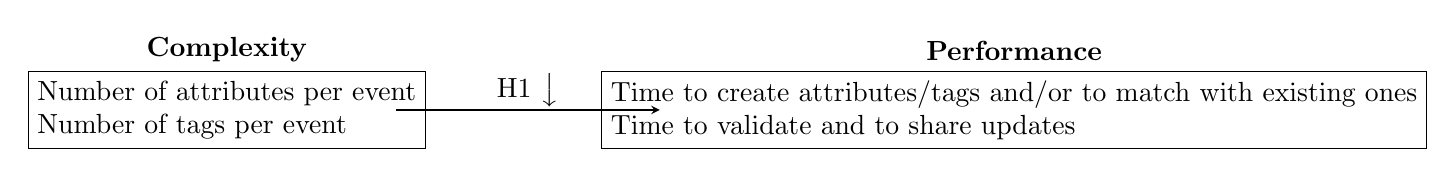
\begin{tikzpicture}
\tikzstyle{container1} = [inner sep=7pt, draw=black!20, rounded corners, line width=0.6mm]
\node[draw, label={{\bf Complexity}}, align=left] at (-5,0) {Number of attributes per event\\ Number of tags per event};
\node[draw, label={{\bf Performance}},align=left] at (5,0) {Time to create attributes/tags and/or to match with existing ones\\Time to validate and to share updates};
\draw [-stealth](-2.85,0) -- (0.5,0);
\node at (-1.175,0.25) {H1 $\big\downarrow$};
\end{tikzpicture}
\caption{Causal diagram relating complexity (left) and performance factors (right) $\downarrow$ indicates a negative effect of the former on the latter.}
\label{fig:H1}
\end{center}
\end{figure}

\subsection{Collective Action Improves Performance (H2)}
 
We consider how collective action at scale positively or negatively affects performance. Namely, there are conflicting views on whether having more stakeholders (e.g., contributors, organizations) joining collective action is likely to enhance or hinder performance \cite{olson_logic_1971, sornette2014much,scholtes_aristotle_2016, maillart_aristotle_2019,muric_collaboration_2019}. Yet, to exist and be sustainable, collective action necessarily needs to bring economies of scale of some form, which in turn would attract more contributors. Figure $\ref{fig:org}$B shows that, over time, organizations join the CIRCL MISP instance following a Poisson process. Upon joining, these organizations immediately benefit from the knowledge accumulated and shared by other organizations, which contributed early on and gained expertise. Also similar or partially similar threats can be treated more efficiently over time, representing economies of scale. Conversely, for new users, learning and familiarizing  with MISP may reduce the performance on the short term {\cite{stojkovski_whats_2021}}, while bringing long-term positive marginal gains. Finally, having more participants should bring marginally increasing performance. We therefore test the following hypothesis:\\

\textbf{H2a}: \textit{The overall performance increases with the number of organizations participating in collective action}.\\

Yet, as already shown in \cite{kuypers_designing_2018}, increased workload is likely to affect negatively performance, and thus, increase the expected completion time. When several threats occur, respectively are open, we posit that completion time of a focal event will necessarily be delayed as a result of priority queuing \cite{maillart_quantification_2011}. We could further hypothesize that given task overload, organizations may resort to increasingly  selfish behavior, by focusing only on their threats and possibly by reducing their information sharing, hence decreasing collective performance \cite{laube_strategic_2017, KOUTSOUPIAS200965}. Therefore, our second hypothesis states:\\

\textbf{H2b}: \textit{Given a focal event, the number of simultaneously open events decreases performance.}\\

\noindent
The hypothesized causality between collective action and performance is shown in Figure $\ref{fig:H2}$.

\begin{figure}[!ht]
\begin{center}
\begin{tikzpicture}
\node[draw, label = {\bf Organizations}, align=left] at (-2, 0.75) (1) {Existing content \\ Expertise of org \\ Software learning};
\node[draw, label = {\bf Simultaneity}, align=left] at (-2, -0.75) (2) {Selfish behavior \\ Information retention};
\node[draw, label={\bf Collective action}, fit margins = {left=1pt,right=1pt,bottom=1pt,top=7pt}, fit = (1) (2)] {};
\draw [-stealth](-0.75,1.15) -- (0.75,1.15);
\draw [-stealth](-0.75,0.75) -- (0.75,0.75);
\draw [-stealth](-0.75,0.35) -- (0.75,0.35);
\node [fill=white] at (0,1.15) {$\uparrow$};
\node [fill=white] at (0,0.75) {$\uparrow$};
\node [fill=white] at (0,0.35) {$\downarrow$};
\draw[-] (0.75,1.15) -- (0.75,0.35) {};
\draw [-stealth](0.75,0.75) -- (2.6,0.75);
\node at (1.675,1) {H2a $\big\uparrow$};
\draw [-stealth](-0.5,-0.6) -- (0.75,-0.6);
\draw [-stealth](-0.5,-1) -- (0.75,-1);
\node [fill=white] at (0,-0.6) {$\downarrow$};
\node [fill=white] at (0,-1) {$\downarrow$};
\draw[-] (0.75,-0.6) -- (0.75,-1) {};
\draw[-] (0.75,-0.8) -- (1,-0.8) {};
\draw[-] (1,-0.8) -- (1,0) {};
\draw [-stealth](1,0) -- (2.6,0);
\node at (1.675,0.25) {H2b $\big\downarrow$};

\node[draw, label={\bf Performance}, align=left] at (7,0.35) {Time to complete an event with help of experts/existing content \\  \\Learning time};

% \draw [-stealth](-2.85,0) -- (0.5,0);
% \node[draw] at (0,0) (n1) {hello};
% \node[draw] at (0,-2) (n2) {hello2};
% \node[draw,fit=(n1) (n2)] {};
% \node at (-1.175,0.25) {H2 $\big\downarrow$};
\end{tikzpicture}
\caption{Causal diagram between the factors of collective action on the left hand side and the factors of performance on the right hand side. $\uparrow$ means an increase of performance, while $\downarrow$ a decrease.}
\label{fig:H2}
\end{center}
\end{figure}

\subsection{Knowledge Integration Increases Performance (H3)}

Having more contributors does not necessarily imply economies of scale \cite{scholtes_aristotle_2016}. Economies of scale may rather be generated by ``the whole is more than the sum of its parts" mechanisms \cite{sornette2014much}, which may stem from productive integration of information  \cite{oizumi_phenomenology_2014, malone_superminds_2018,engel_integrated_2018} as a single entity \cite{sornette2014much} or through the efficient communication of several modular sub-systems \cite{barrett_practical_2011,baldwin_design_2000}, which in turn may even mitigate free-riding \cite{baldwin_architecture_2006}. Here, we recognize that the first form on knowledge integration occurs through experience as {\it learning}, through regular software use, repeated resolution processes of numerous events and interactions with other participating organizations and their users within organizations \cite{argote_organizational_2011}. An organization having accumulated experience in characterizing a large number of threat events is likely to perform better on new events, therefore:\\

\textbf{H3a}: \textit{More experienced organizations to faster event resolution.}\\

On MISP instances, collective action goes beyond coordinating time-critical tasks. As people and organizations contribute, a large corpus of knowledge is built as a library of events, attributes, and tags. In turn, by design of MISP software, this information can be easily reused to quickly characterize new events, proposing matching possibilities according to the preliminary entries. Hence,  reuse of knowledge simplifies the emission of attributes and the knowledge is integrated by the creator of the new events. These new events are thus composed of a certain percentage of {\it inherited} attributes which are likely to impact positively performance:\\ 

\textbf{H3b}: \textit{Reuse of tags and attributes from existing events contributes positively to performance in the completion of new events.}\\

The capacity of an entity to integrate knowledge is tightly related to its modular organization \cite{tononi_consciousness_1998,narduzzo_role_2005,baldwin_architecture_2006}. As MISP clusters of events or attributes, called ``Galaxies", were progressively introduced and developed on MISP CIRCL, we have an opportunity to test for modularity. Indeed, events or attributes can be attached to one or several Galaxies according to key values (e.g., their type, tags, category, distribution level and/or threat level) associated with a given level of granularity, which is proportional to its prevalence in the MISP ecosystem (c.f., Appendix A). Therefore, a higher granularity refers to higher specificity, which in turn, goes against performance. Conversely, a key value that would be too general, would not provide discriminate information, and therefore would go against performance {\cite{west2016impact}}. Modularity provides a good balance between too fine-grained and too coarse-grained. We therefore formulate the following hypothesis:\\

\textbf{H3c}: \textit{Modularity in collective action positively influences performance.}\\

\noindent
Figure $\ref{fig:H3}$ shows the causality relationships between knowledge integration factors and performance.

\begin{figure}[!ht]
\begin{center}
\begin{tikzpicture}
\node[draw, label = {\bf Experience}, align=left] at (-2, 1.6) (1) {Regular software use \\ Repetition of resolution processes \\ In-depth knowledge of threats};
\node[draw, label = {\bf Reuse of content}, align=left] at (-2, 0) (2) {Availability of existing content \\ Match by criteria \\ Errors in the content};
\node[draw, label = {\bf Modularity}, align=left] at (-2, -1.5) (3) {Referral to reliable content \\ Granularity};
\node[draw, label={\bf Knowledge integration}, fit margins = {left=1pt,right=1pt,bottom=1pt,top=7pt}, fit = (1) (3)] {};
\draw [-stealth](0.3,2) -- (1.95,2);
\draw [-stealth](0.3,1.6) -- (1.95,1.6);
\draw [-stealth](0.3,1.2) -- (1.95,1.2);
\node [fill=white] at (1.125,2) {$\uparrow$};
\node [fill=white] at (1.125,1.6) {$\uparrow$};
\node [fill=white] at (1.125,1.2) {$\uparrow$};
\draw [-stealth](0.1,0.35) -- (1.95,0.35);
\draw [-stealth](0.1,-0.05) -- (1.95,-0.05);
\draw [-stealth](0.1,-0.45) -- (1.95,-0.45);
\node [fill=white] at (1.125,0.35) {$\uparrow$};
\node [fill=white] at (1.125,-0.05) {$\uparrow$};
\node [fill=white] at (1.125,-0.45) {$\downarrow$};
\draw [-stealth](-0.12,-1.3) -- (1.95,-1.3);
\draw [-stealth](-0.12,-1.7) -- (1.95,-1.7);
\node [fill=white] at (1.125,-1.3) {$\uparrow$};
\node [fill=white] at (1.125,-1.7) {$\uparrow$ $\downarrow$};
\draw[-] (1.95,2) -- (1.95,1.2) {};
\draw[-] (1.95,0.35) -- (1.95,-0.45) {};
\draw[-] (1.95,-1.3) -- (1.95,-1.7) {};
\node at (3.275,0.2) {H3b $\big\uparrow$};
\draw [-stealth](1.95,-0.05) -- (4.6,-0.05);
\draw[-] (1.95,1.6) -- (3.75,1.6) {};
\draw[-] (3.75,1.6) -- (3.75,0.7) {};
\draw [-stealth](3.75,0.7) -- (4.6,0.7);
\node at (3.275,1.85) {H3a $\big\uparrow$};
\draw[-] (1.95,-1.5) -- (3.75,-1.5) {};
\draw[-] (3.75,1.6) -- (3.75,0.7) {};
\draw [-stealth](3.75,-0.8) -- (4.6,-0.8);
\draw[-] (3.75,-1.5) -- (3.75,-0.8) {};
\node at (3.275,-1.25) {H3c $\big\uparrow$};
\node[draw, label={\bf Performance}, align=left] at (7,0) {Time to solve events faster\\ \\ Increasing knowledge over time \\ \\ Orientation toward reliable content};
\end{tikzpicture}
\caption{Causal diagram between the factors of knowledge integration on the left hand side and the factors of performance on the right hand side. $\uparrow$ means an increase of performance, while $\downarrow$ a decrease.}
\label{fig:H3}
\end{center}
\end{figure}


By testing these three hypotheses (and six sub-hypotheses), we expect to gain robust insights on how collective action on MISP brings performance in terms of characterizing time-critical cybersecurity threats. Figure $\ref{fig:H}$ illustrates the expected influence of event complexity, collective action and knowledge integration on the time needed to complete the characterization of threats events.

\begin{figure}[!ht]
\begin{center}
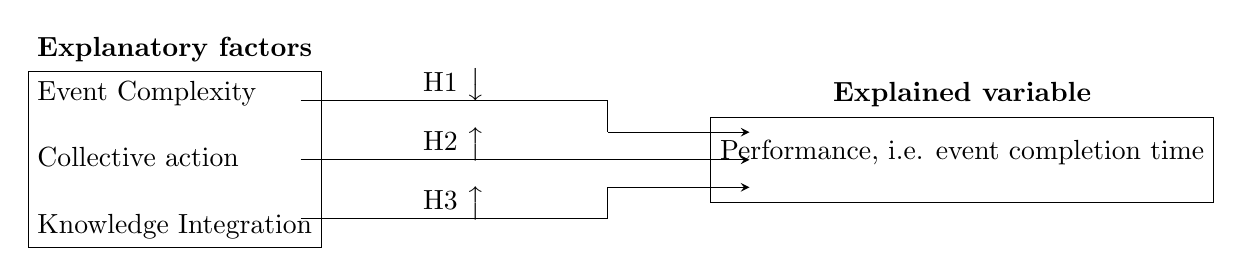
\begin{tikzpicture}
\node[draw, label={{\bf Explanatory factors}}, align=left] at (-5,  0) {Event Complexity\\ \\ Collective action\\ \\ Knowledge Integration};
\node[draw, label={{\bf Explained variable}}, align=left] at (5,  0) { \\ Performance, i.e. event completion time \\ };
\draw [-](-3.4,0.75) -- (0.5,0.75);
\draw [-stealth](0.5,0.35) -- (2.3,0.35);
\draw [-](0.5,0.75) -- (0.5,0.35);
\draw [-stealth](-3.4,0.0) -- (2.3,0.0);
\draw [-](-3.4,-0.75) -- (0.5,-0.75);
\draw [-stealth](0.5,-0.35) -- (2.3,-0.35);
\draw [-](0.5,-0.75) -- (0.5,-0.35);
\node at (-1.45,0.95) {H1 $\big\downarrow$};
\node at (-1.45,0.2) {H2 $\big\uparrow$};
\node at (-1.45,-0.55) {H3 $\big\uparrow$};

\end{tikzpicture}
\caption{Causal diagram between the explanatory factors on the left hand side and the explained variable of performance, namely event completion time on the right hand side. $\uparrow$ means an increase of performance, while $\downarrow$ a decrease.}
\label{fig:H}
\end{center}
\end{figure}

\section{Method}
\label{sec:method}

We proceed to validate our theory through the testing of three hypotheses, divided in six sub-hypotheses (c.f., ``\hyperref[sec:hypotheses]{Hypotheses}" section).  For this, we specify an econometric model with {\it completion time} as the main dependent variable representing the key performance indicator in our posited {\it theory of collective action for tackling time-critical threats} (c.f.,  ``\hyperref[sec:theory]{Theoretical Framework}" section).

We define the following set of events,

\begin{align}
    \Omega_e = \{e|e \leq N_e, e \in \mathbb{N}^{\ast}\},
\end{align}
\noindent
where $N_e$ corresponds to $22\,423$ events, which have explicitly been marked as completed (i.e., with field $Analysis = 2$, see ``\hyperref[sec:data]{Data}" section). For each event, we define $\Delta t_{C,e}$ the completion time of events as 
\begin{equation}
    \Delta t_{C,e} = t_{f,e} - t_{c,e},
\end{equation} 
\noindent
with $t_{c,e}$ the event creation date and $t_{f,e}$ the last event modification.  

To determine the relation between the dependent variable, i.e. the completion time $\Delta t_{C,e}$ for the events, we proceed to a multivariate cross-sectional regression \cite{asteriou_applied_2015}. Specifically, we investigate if completion time $\Delta t_{C,e}$ for the events can be explained by the selected explanatory variables. The corresponding \texttt{Python} variable is \texttt{CompletionT}. For each event $e$, the multivariate cross-sectional regression writes:

\begin{align}
    \log(\Delta t_{C,e}) &= \zeta + \sum_{k=1}^{N_k} \cdot \sum_{e=1}^{N_e} \kappa_{k} \cdot \log(Z_{k,e}) + \varepsilon_e,
    \label{eq:EcoModel}
\end{align}
\noindent
with:
\begin{quote}
   \begin{itemize}
       \item[--] $\Delta t_{C_e}$ : time completion for event $e$, 
       \item[--] $\zeta$ : constant,
        \item[--] $N_k$ : number of explanatory variables,
       \item[--] $\kappa_{k}$ : autoregressor parameter  corresponding to $Z_{k,e}$,
       \item[--] $Z_{k,e}$ : k-th explanatory variable for event $e$,
       \item[--] $\varepsilon_e$ : error term (i.e., $\log(\Delta t_{C,e}) - \log(\widehat{\Delta t_{C,e}})$). 
   \end{itemize}
\end{quote}

This multivariate cross-sectional regression is performed with the ordinary least squares (OLS) method. The choice of this model is  adapted to deal with data without time series, which is the case here. Then, the explicated and explanatory variables are linked with a set of points in time. This set of points in time is given by the creation $t_{c,e}$ of the different $e$ and contains $22\,423$ elements, corresponding to the number of completed elements $N_e$ considered.  
Thanks to this model, it is easy to consider all chosen independent variables. However, due to the heavy-tailed behaviour of the variables and their difference of magnitude (see ``\hyperref[sec:data]{Data}" section), we transform the variables in logarithm in base of 10 \cite{benoit_linear_2011}. However, the results are indicated as a percentage change of $\Delta t_{C,e}$ when $Z_{k,e}$ varies by a certain percentage \cite{benoit_linear_2011}.

We specify the following explanatory variables in relation with the formulated hypotheses (c.f., ``\hyperref[sec:hypotheses]{Hypotheses}" section). To test hypothesis {\bf H1} (i.e., {\it event complexity hinders performance}), we resort to two explanatory variables:
\begin{quote}
\begin{itemize}
    \item[--] $N_{A,e}$: the number of attributes per event $e$. The corresponding \texttt{Python} variable is \texttt{AttrCount}, which is expected to positively influence \texttt{CompletionT} (i.e., reduce performance).
    \item[--] $N_{T,e}$: the number of tags per event $e$, The corresponding \texttt{Python} variable is \texttt{NTags}, which is expected to positively influence \texttt{CompletionT} (i.e., reduce performance). 
\end{itemize}
\end{quote}

To test hypothesis {\bf H2} (i.e., {\it collective action improves performance}), we resort to two explanatory variables:

\begin{quote}
\begin{itemize}
\item[--]$N_{O,e}$ stands for the number of organizations listed on MISP CIRCL at the creation $t_{c,e}$ of event $e$. The corresponding \texttt{Python} variable is \texttt{CumOrgs}. \texttt{CumOrgs} is expected to negatively influence \texttt{CompletionT} (i.e., increase performance) and to demonstrate the overall benefits of collective action for tackling time criticial threats ({\bf H2a}). 
\item[--] $E_{\textrm{sim},e}$ is the number of simultaneously open events on MISP CIRCL at the creation $t_{c,e}$ of event $e$. The corresponding \texttt{Python} variable is \texttt{SimEvents}, which is expected to positively influence \texttt{CompletionT} (i.e., reduce performance) and to show that collective action performance is bound to circumstantial operational constraints associated with time as a scarce resource ({\bf H2b}) \cite{maillart_quantification_2011,kuypers_designing_2018}.
\end{itemize}
\end{quote}


To test hypothesis {\bf H3} (i.e., {\it knowledge integration increases performance}), we resort to three explanatory variables:


\begin{quote}
\begin{itemize}
    \item[--] $E_{C,e}$ takes into account the number of already completed events by the organizations at the creation $t_{c,e}$ of a new event $e$ on their behalf. The corresponding \texttt{Python} variable is \texttt{CumCompE}, which is expected to negatively influence \texttt{CompletionT} (i.e., increase performance) ({\bf H3a}).
    \item[--] $I_{{\%A},e}$ is the inherited percentage of attributes per event $e$. The corresponding \texttt{Python} variable is \texttt{InhPer}, which is expected to negatively influence \texttt{CompletionT} (i.e., increase performance) ({\bf H3b}).
    \item[--] $N_{G,e}$ counts the number of galaxies created on MISP CIRCL instance at the creation $t_{c,e}$ of the $e$. The corresponding \texttt{Python} variable is \texttt{NbGalaxies}, which is expected to negatively influence \texttt{CompletionT} (i.e., increase performance)  ({\bf H3c}). 
    \item[--] $N_{E_G,e}$ considers the number of events in its corresponding aforementioned galaxy at the creation $t_{c,e}$ of a new event $e$ in this galaxy. The corresponding \texttt{Python} variable is \texttt{NbEventsinhisG}, which is expected to negatively influence \texttt{CompletionT} (i.e., increase performance)  ({\bf H3c}).
\end{itemize}
\end{quote}

The pairwise correlations of the dependent variable and the independent ones provide the correlation matrix (see Table \ref{tab:CorrM}).

With the explanatory variables of our model being defined, we are in position to formulate the econometric model by developing the equation $\eqref{eq:EcoModel}$:

\begin{align}
    \log(\Delta t_{C,e}) = \zeta &+ \kappa_{N_A} \cdot \log(N_{A,e}) + \kappa_{I_{\%A}} \cdot \log(I_{\%A, e}) + \kappa_{N_T} \cdot \log(N_{T,e}) \nonumber\\ 
    &+ \kappa_{E_\textrm{sim}} \cdot \log(E_{\textrm{sim},e}) + \kappa_{N_O} \cdot \log(N_{O,e}) + \kappa_{E_C} \cdot \log(E_{C,e}) \nonumber\\
    &+ \kappa_{N_G} \cdot \log(N_{G,e}) + \kappa_{N_{E_G}} \cdot \log(N_{E_G,e}) \nonumber\\
    &+ \varepsilon_e 
\label{eq:OLS1}
\end{align}\\


    
    
    Model validation is performed as follows. When handling a multivariate regression, one must pay particular attention to  multi-collinearity between the $Z_k$'s, which may distort the model. For that, the variance inflation factor (VIF) resulting from the regression of the explanatory variable $Z_k$ on the other explanatory variables which provide $R_{k}^2$, must be computed. The $\textrm{VIF}_k$ is then given as $\textrm{VIF}_k = 1/(1-{R_k}^2)$ and must be $< 10$ \cite{asteriou_applied_2015}. The stability of the variance has to be examined, namely by studying heteroskedasticity, which is ruled out if the $p$-value obtained from a White test is lower than a threshold $\alpha = 0.05$ \cite{asteriou_applied_2015}. The computation steps are performed with the \verb?Python? libraries \verb?statsmodels.api.OLS? for the regression, \verb?statsmodels.stats.outliers_influence? for the VIF and \verb?statsmodels.stats.diagnostic? for the White test.

\section{Results}
\label{sec:results}
In order to establish evidence of collective action as an efficient way for tackling time-critical cybersecurity threats, we have resorted to data the MISP instance, which is run by the computer Incident Response Center Luxembourg (CIRCL). We used  a multivariate cross-sectional regression analysis of {\it completion time} (i.e., performance) required to characterize a threat event with both event related and collective action explanatory variables. 

The regression results are shown in Table \ref{tab:OLS Stats}. Overall, the regression model is robust and explains $41.3\%$ of the variance ($R^2 = 0.413$). Testing for hypothesis 1, the model shows that indeed event complexity measured by the number of attributes \texttt{CountAttr} and tags \texttt{NTags} influences performance negatively, i.e., event characterization completion time is increased. Hypothesis H1 is supported. Regarding how collective action improves performance (H2), the model shows that overall performance (i.e., completion time reduced) is positively associated with the number of organizations participating in MISP: Hypothesis H2a is supported. Hypothesis H2b could not be tested as a result of unexplained strong multi-collinearity between \texttt{CumOrgs} and \texttt{SimEvents}. Turning to Hypothesis 3 (i.e., knowledge integration increases performance), we find that more experienced organizations perform better in reducing event completion time. Hypothesis H3a is supported. We also find that the proportion of attributes that an event $e$ inherits from previous events, i.e., from the MISP CIRCL knowledge base, also positively influences performance. Hypothesis H3b is supported. Finally, testing for hypothesis H3c, i.e., modularity, we find mixed results. While the number of MISP Galaxies, measuring the number of modular sub-systems, influences positively performance, the number of events recorded in MISP Galxies, measuring to some extent the intensity of modularity, influences performance negatively. Hypothesis H3b is only partially supported.

 We have checked for multi-collinearity of the explanatory variables. We computed the variance inflation factor (VIF) for each explanatory variables, which happens to be all smaller than 10. This implies that there is no evidence of multi-collinearity between the selected explanatory variables (c.f., Table \ref{tab:VIF}). We also controlled for heteroskedasticity, i.e., a possible instability of the variance by performing a White statistics tests. We obtained $p\textrm{-value} < 10^{-2}$, which implies that there is no heteroskedasticity in our model. The post-analysis for the VIFs and the White statistics test completely validate the used model and its results.

\section{Discussion}
\label{sec:discussion}
Organizations are increasingly encouraged to cooperate and share information to overcome cybersecurity threats. Investigating how collective action unfolds and brings performance on information-sharing platforms is necessary as cybersecurity threats have become increasingly time-critical. Organizations shall resort to collective action to gather information and integrate knowledge as two pillars of threat event characterization not only as attacks unravel, but also before attacks unravel \cite{wagner_cyber_2019}. Here, we have investigated collective action on MISP, a popular open source threat intelligence platform, from the perspective of the time required to fully characterize an event as the objective function for performance. We found that performance is negatively associated with event complexity (Hypothesis 1) and positively associated with collective action (Hypothesis 2). Indeed, as the number of organizations taking part to information-sharing on the studied MISP instance, the time required to complete the characterization of events decreased. This result informs on positive returns on scale, which necessarily exist given the increased adoption of MISP as well as other information-sharing platforms. Nevertheless, the mechanisms at work generating these economies of scale have remained unclear. We considered the perspective of knowledge integration \cite{tononi_consciousness_1998} as the collective action process at work to generate the ``the whole is more than the sum of its parts" \cite{sornette2014much}. With Hypothesis 3, we tested and verified organizational learning, knowledge integration and modularity as being positively associated with performance.\\

While event completion time is associated with explanatory variables pertaining to event complexity, collective action, and knowledge integration, we could not establish causality. Although this is a significant limitation to our model, we have organized our multivariate cross-sectional regression in a way that minimizes the risks of uncovering spurious dependencies between the explained variable on the one hand and the explanatory variables on the other hand. To the exception of \texttt{SimEvents},i.e., the number of simultaneously open events on MISP CIRCL at the creation, which had to be excluded from the model, all our explanatory variables are significant. This shows that our proposed theory on {\it collective action for tackling time-critical tasks} is comprehensive and altogether robust. Yet, the regression analysis approach remains exploratory. Indeed, it does not provide reliable information on which precise collective action mechanisms generate positive returns on scale. Building and testing fine-grained causal models of critical cascades in collective action, inspired from e.g. \cite{sornette2014much,maillart_aristotle_2019,muric_collaboration_2019}, may surely help better understand the activity, learning, knowledge integration and modularization paths of contributing organizations, as well as how they handle time as a particularly scarce resource \cite{maillart_quantification_2011}. Indeed, when tackling large amounts of time-critical tasks, such as cybersecurity threats or incidents, contingencies necessarily appear \cite{kuypers_designing_2018}, which may affect coordination between contributors, and performance as a result, either in a transient way or by triggering long-term instability through cascades of disorganization. At the meso-scale, our model does not account for affinities between events, organizations and the combined commonalities of events and organizations. Indeed, as for number of collective action online platforms, modular {\it Galaxies} on MISP show that some sub-communities of organizations have specific goals when tackling cybersecurity threats. These specific interests deserve further scrutiny. For instance, are the organizations contributing to a given MISP galaxy active in the same industry? If not, why do they share interest in similar threats? Considering MISP (or other information-sharing platforms) from the perspective of threats, one may investigate kinship between threats, as many events share attributes. Questioning and perhaps predicting how attributes are ``transmitted" from one event to others is likely to be key to anticipate threats and guide organizations in their search of (respectively contributions to) threat information. It may even help decide what information should be shared and with whom.

Finally, our results show that completion time as an objective function in collective action concerned with time-critical tasks can be optimized. For that purpose, establishing causality between complexity, collective action, modularity factors and performance would certainly help refine the entangled determinants of performance. Further, our our results open further perspectives for computational social science research. One may envision to use machine learning in order to recommend personalized precision strategies that optimize the organization of collective action and knowledge integration. This may help make best use of time as an increasingly critically scarce resource, especially in face of a looming tsunami of cybersecurity threats. Consequently, the increasing adoption of MISP, or equivalent information sharing platforms by more and more of critical infrastructures and of organizations, as evident in our data, further emphasizes their relevance and, in turn, the positive externalities associated with more organizations joining. Notably, MISP's effectiveness in catering to the needs of small and medium businesses adds to the value proposition {\cite{van2021shared}}, even though the efficiency of information sharing platforms for organizations remains to be tested against their size. By merging and modularizing diverse sources of information, such as different communities or instances, we anticipate an enhancement in time performance due to the improved situational awareness, ultimately optimizing information sharing efficiency, and hence making information sharing platforms increasingly attractive.

\section{Conclusion}
\label{sec:conclusion}
Information-sharing in cyber-security has become an increasingly common collective action practice. Yet, its benefits have so far remained unclear. We have investigated MISP, a commonly used open source threat sharing platform, and we found how building a critical mass of contributing organizations and of knowledge to be integrated from past threats brings significant economies of scale. Through collective action, security researchers overcome the challenge of characterizing cybersecurity threats, which appear to be increasingly time-critical. We find that performance, defined as the time needed to fully characterize a threat event, is (i) negatively influenced its own complexity, (ii) positively influenced by collective action, and (iii) positively by learning, knowledge integration and modularity. Our results also inform more generally on how collective action can be organized online at scale and in a modular way to overcome a large number of time-critical tasks.

\section*{Data Availability Statements}
The data underlying this article cannot be shared publicly due to compliant reasons and the limited access to the MISP CIRCL community. A request for access can be made to MISP CIRCL.The code is published open source at the following URL: \url{https://github.com/technometrics-lab/9-Cyber-threats-Intelligence}.


\section*{Acknowledgements}
The authors thank the WEIS’2021, the WEIS’2022  anonymous reviewers, as well as the participants of the WEIS'2022 conference in Tulsa, USA, for their comments. The authors also acknowledge useful comments from reviewers and the Journal of Cybersecurity editor.

The authors acknowledge support from the members of the Computer Incident Response Center Luxembourg (CIRCL) for making their data available and for their technical support. One of the authors (S. Gillard) acknowledges financial support from the Military Academy at ETH Zurich. Two authors (D. Percia David and T. Maillart) acknowledge financial support from the Cyber-Defence Campus (armasuisse Science and Technology).


\bibliographystyle{unsrt}
%\bibliography{reference}

\begin{thebibliography}{10}

\bibitem{sridhar_cybersecurity_2021}
Sridhar, K, Householder, A, Spring, J {\em et al.}
  Cybersecurity Information Sharing: Analysing
an Email Corpus of Coordinated Vulnerability
Disclosure. In: {\em The 20th Annual Workshop on
the Economics of Information Security, Online}, 2021.

\bibitem{gal-or_economic_2005}
Gal-Or, E,  Ghose, A. The Economic Incentives for Sharing Security Information. 
{\em Information Systems Research} 2005; {\bf 16}: 186-208.

\bibitem{maillart_given_2017}
Maillart, T,  Zhao, M, Grossklaggs, J {\em et al.} Given enough eyeballs, all bugs are
shallow? Revisiting Eric Raymond with bug bounty programs. {\em Journal of Cybersecurity} 2017; {\bf 3}: 81-90.

\bibitem{sridhar_hacking_2021}
Sridhar, K, Ng, M. Hacking for good: Leveraging HackerOne
data to develop an economic model of Bug Bounties. {\em Journal of Cybersecurity} 2021; {\bf 7}: 1-9.

\bibitem{bohme_back_2016}
B\"{o}hme, R. Back to the Roots: Information Sharing Economics and What We Can Learn for Security. In: {\em Proceedings of the 2016 ACM on Workshop on Information
Sharing and Collaborative Security, Vienna Austria,} 2016. p.1-2.

\bibitem{laube_strategic_2017}
Laube, S, B\"{o}hme, R. Strategic Aspects of Cyber Risk Information Sharing. {\em ACM Computing Surveys} 2017; {\bf 50}(77): 1-36.

\bibitem{brady_murphys_1999}
Brady, RM, Anderson, RJ, Ball, RC. Murphy’s law, the fitness of evolving species, and the limits of software reliability. {\em University of Cambridge, Computer Laboratory} 1999, 10.48456/tr-471.

\bibitem{stojkovski_whats_2021}
Stojkovski, B, Lenzini, G, Koenig, V {\em et al.} What’s in a Cyber Threat Intelligence
sharing platform?: A mixed-methods user experience investigation of MISP. In: {\em Annual Computer Security Applications Conference, Virtual Event,} 2021. p. 385-398.

\bibitem{levy_hackers_2010}
Levy, S. Hackers: {\em Heroes of the computer revolution}. New York: Anchor Press/Doubleday, 1984.

\bibitem{benkler_penguin_2011}
Benkler, Y. {\em The Penguin and the Leviathan: How Cooperation Triumphs over Self-Interest.} Currency, 2011.

\bibitem{benkler_wealth_2006}
Benkler, Y. {\em The wealth of networks: how social production transforms markets and
freedom.} New Heaven: Yale University Press, 2006.

\bibitem{katz_network_1985}
Katz, ML, Shapiro, C. Network externalities, competition, and compatibility. {\em The American economic review} 1985; {\bf 75}(3): 424-440.

\bibitem{shapiro_information_1999}
Shapiro, C, Varian, HR. {\em Information rules: a strategic guide to the network economy.} Boston: Harvard Business School Press, 1999.

\bibitem{wagner_misp_2016}
Wagner, C, Delaunoy, A, Wagener, G {\em et al.} MISP: The Design and Im-
plementation of a Collaborative Threat Intelligence Sharing Platform. In: {\em Proceedings
of the 2016 ACM on Workshop on Information Sharing and Collaborative Security, New York NY,} 2016. p. 49-56. Association for Computing Machinery, New York, NY, USA.

\bibitem{zibak_cyber_2019}
Zibak, A, Simpson, A. Cyber Threat Information Sharing: Perceived Benefits and Barriers. In: {\em Proceedings of the 14th International Conference on Availability,
Reliability and Security} 2019. p. 1-9. ACM, Canterbury, CA, UK.

\bibitem{mell_common_2006}
Mell, P, Scarfone, K, Romanosky, S. Common Vulnerability Scoring System. {\em IEEE Security \& Privacy} 2006; {\bf 4}(6): 85-89.

\bibitem{olson_logic_1971}
Olson, M. {\em The Logic of Collective Action: Public Goods and the Theory of Groups,
With a New Preface and Appendix.} Cambridge: Harvard University Press, 1971.

\bibitem{anesi_moral_2009}
Anesi, V. Moral hazard and free riding in collective action. {\em Social Choice and Welfare} 2009; {\bf 32}: 197-219.

\bibitem{esteban_collective_2001}
Esteban, J, Ray, D. Collective action and the group size paradox. {\em American political science review} 2001; {\bf 95}(3): 663-672.

\bibitem{varian2004system}
Varian, HR. System Reliability and Free Riding. In: Economics of information security. Boston: Springer, 2004, 1-15.

\bibitem{dejean_olsons_2010}
Dejean, S, P\'enard, T, Suire, R. Olson’s Paradox Revisited: An Empirical Analysis
of incentives to contribute in P2P File-Sharing Communities. {\em SSRN} 2010, 10.2139/ssrn.1299190.

\bibitem{KOUTSOUPIAS200965}
Koutsoupias, E, Papadimitriou, C. Worst-case equilibria. In: Meinel, C, Tison, S (ed). {\em STACS 1999.} Berlin: Springer, 1999, 404-413.

\bibitem{asvanund_empirical_2004}
Asvanund, A, Clay, K, Krishnan, R {\em et al.} Empirical Analysis of Network Externalities in Peer-to-Peer Music-Sharing Networks. {\em Information Systems
Research} 2004; {\bf 15}: 155-174

\bibitem{klein_virtuous_2015}
Klein, M, Maillart, T, Chuang, J. he Virtuous Circle of Wikipedia: Recursive Measures of Collaboration Structures. In: {\em Proceedings of the 18th ACM Conference on Computer Supported Cooperative Work \& Social Computing, Vancouver BC,} 2015. p. 1106-1115. Association for Computing Machinery, New York, NY, USA.

\bibitem{wang_empirical_2013}
Wang, S, Lo, D, Jiang, L. An empirical study on developer interactions in Stack-Overflow. In: {\em Proceedings of the 28th Annual ACM Symposium on Applied Computing, 	Coimbra,} 2013. p. 1019-1024. Association for Computing Machinery, New York, NY, USA. 

\bibitem{hippel_open_2003}
Hippel, Ev, Krogh, Gv. en Source Software and the “Private-Collective” Innovation Model: Issues for Organization Science. {\em Organization Science} 2003; {\bf 14}(2): 209-223.

\bibitem{sornette2014much}
Sornette, D, Maillart, T, Ghezzi, G. How much is the whole really more than the
sum of its parts? $1 \boxplus 1 = 2.5$: Superlinear productivity in collective group actions. {\em PLoS ONE} 2014, 10.1371/journal.pone.0103023.

\bibitem{maillart_aristotle_2019}
Maillart, T, Sornette, D. Aristotle vs. Ringelmann: On superlinear production in open source software. {\em Physica A: Statistical Mechanics and its Applications} 2019; {\bf 523}: 964-972

\bibitem{muric_collaboration_2019}
Muri\'c, G, Abeliuk, A, Lerman, K {\em et al.} Collaboration Drives Individual Productivity. {\em Proceedings of the ACM on Human-Computer Interaction} 2019; {\bf 3}: 1-24.

\bibitem{scholtes_aristotle_2016}
Scholtes, I, Mavrodiev, P, Schweizer, F. From Aristotle to Ringelmann: a large-scale analysis of team productivity and coordination in Open Source Software projects. {\em Empirical Software Engineering,} 2016; {\bf 21}(2): 642-683.

\bibitem{tziner_effects_1985}
Tziner, A, Eden, D. ffects of crew composition on crew performance: Does the whole equal the sum of its parts? {\em Journal of Applied Psychology} 1985; {\bf 70}(1): 85-93.

\bibitem{sundstrom_work_1990}
Sundstorm, E, De Meuse, KP, Futrell, D. Work teams: Applications and effectiveness. {\em American Psychologist} 1990; {\bf 45}(2): 120-133.

\bibitem{cohen_what_1997}
Cohen, SG, Bailey DE. What Makes Teams Work: Group Effectiveness Research from the Shop Floor to the Executive Suite. {\em Journal of Management} 1997; {\bf 23}(3): 239-290.

\bibitem{neuman_team_1999}
Neumann, GA, Wright, J. am effectiveness: Beyond skills and cognitive ability. {\em Journal of Applied Psychology} 1999; {\bf 84}(3): 376.

\bibitem{ennen_whole_2010}
Ennen, E, Richter, A. The Whole Is More Than the Sum of Its Parts— Or Is It? A Review of the Empirical Literature on Complementarities in Organizations. {\em Journal of Management} 2010; {\bf 36}(1): 207-233.

\bibitem{sacramento_team_2006}
Sacramento, CA, Chang, MWS, West, MA. Team Innovation through Collaboration. In: Beyerlein, MM, Beyerlein, ST and Kennedy, FA (ed). {\em Innovation through Collaboration.} Bingley: Emerald Group Publishing Limited, 2006, 81-112.

\bibitem{nonaka_dynamic_1994}
Nonaka, I. A Dynamic Theory of Organizational Knowledge Creation. {\em Organization Science} 1994; {\bf 5}(1): 14-37.

\bibitem{grant_prospering_1996}
Grant, RM. Prospering in Dynamically-Competitive Environments: Organizational Capability as Knowledge Integration. {\em Organization Science} 1996; {\bf 7}(4): 375-387.

\bibitem{wuchty_increasing_2007}
Wuchty, S, Jones, BF, Uzzi, B. The Increasing Dominance of Teams in Production of Knowledge. {\em Science} 2007; {\bf 316}(5827) 1036-1039.

\bibitem{lawrence_differentiation_1967}
Lawrence, PR, Lorsch, JW. Differentiation and Integration in Complex Organizations. {\em Administrative Science Quarterly} 1967; {\bf 12}(1): 1-47.

\bibitem{majchrzak_catalyst_2018}
Majchrzak, A, Griffith, TL, Reetz, DK {\em et al.} Catalyst Organizations as a New Organization Design for Innovation: The Case of Hyperloop Transportation Technologies. {\em Academy of Management Discoveries} 2018; {\bf 4}(4): 472-496.

\bibitem{safa_information_2016}
Safa, NS, Von Solms, R. An information security knowledge sharing model. {\em Computers in Human Behavior} 2016; {\bf 57}: 442-451.
in organizations.

\bibitem{mockus_case_2000}
Mockus, A, Fielding, RT, Herbsleb, J. A case study of open source software development: the Apache server. In: {\em Proceedings of the 22nd international conference on Software engineering, Limerick Ireland,} 2000. p.263-272. Association for Computing Machinery, New York, NY, USA.

\bibitem{kenneth_j_arrow_and_gerard_debreu_existence_1954}
Arrow, KJ, Debreu, G. Existence of an Equilibrium for a Competitive Economy. {\em The Econometric Society} 1954; {\bf 22}(3): 265-290.

\bibitem{ravasi_organising_2001}
Ravasi, D, Verona, G. Organising the process of knowledge integration: the benefits of structural ambiguity. {\em Scandinavian Journal of Management} 2001; {\bf17}(1): 41-66.

\bibitem{huang_knowledge_2003}
Huang, JC, Newell, S. Knowledge integration processes and dynamics within the context of cross-functional projects. {\em International journal of project management} 2003; {\bf21}(3): 167-176.

\bibitem{engel_integrated_2018}
Engel, D, Malone, TW. Integrated information as a metric for group interaction. {\em PLoS ONE} 2018, 10.1371/journal.pone.0205335.

\bibitem{tononi_consciousness_1998}
Tononi, G. Consciousness and Complexity.{\em Science} 1998; {\bf 282}(5395): 1846-1851.

\bibitem{zheng_cyber_2015}
Zheng, DE, James, A. {\em Cyber Threat Information Sharing: Recommendations for Congress and
the Administration.} Washington DC: Center for Strategic \& International Studies, 2015

\bibitem{he_perspectives_2018}
He, M, Devine, L, Zhuang, J. Perspectives on Cybersecurity Information Sharing
among Multiple Stakeholders Using a Decision-Theoretic Approach: Cybersecurity Information Sharing. {\em Risk Analysis} 2018; {\bf 38}(2): 215–225

\bibitem{meier_feedrank_2018}
Meier, R, Scherrer, C, Gugelmann, D {\em et al.} FeedRank: A tamper-resistant method for the ranking of cyber threat intelligence feeds. In: {\em 10th
International Conference on Cyber Conflict (CyCon), Tallinn}, 2018. p. 321-344. NATO Cooperative Cyber Defence Centre of Excellence, Tallinn, Estonia.

\bibitem{mermoud_share_2019}
Mermoud, A, Keupp, MM, Huguenin, K {\em et al.} Toshare or not to share: a behavioral perspective on human participation in security
information sharing. {\em Journal of Cybersecurity} 2019; {\bf 5}: 1-13.

\bibitem{perciadavid_knowledge_2020}
Percia David, D, Keupp, MM, Mermoud, A. Knowledge absorption for cybersecurity: The role of human beliefs. {\em Computers in Human Behavior} 2020, 10.1016/j.chb.2020.106255.

\bibitem{mermoud_governance_2019}
Mermoud, A, Keupp, MM, Percia David, D. Governance Models Preferences for Security Information Sharing: An Institutional Economics Perspective for Critical
Infrastructure Protection. In: Luiijf, E, \v{Z}utautait\.{e}, I, H\"ammerli, B (ed). {\em Critical Information Infrastructures Security (CRITIS) 2018}. Cham: Springer, 2019, 179-190.

\bibitem{oliver_reward_1980}
Oliver, P. Rewards and Punishments as Selective Incentives for Collective Action: Theoretical Investigations. {\em American journal of sociology} 1980; {\bf 85}(6): 1356-1375.

\bibitem{hirshleifer_weakest-link_1983}
Hirshleifer, J. From weakest-link to best-shot: The voluntary provision of public goods. {\em Public choice} 1983; {\bf 41}(3): 371-386.

\bibitem{mermoud_three_2019}
Mermoud, A. Three articles on the behavioral economics of security information
sharing: A theoretical framework, an empirical test, and policy recommendations. {\em PhD. Thesis.} University of Lausanne Faculty of Business and Economics 2019.

\bibitem{bouwman_governance_2018}
Bouwman, X. Governance of cybersecurity communities: Understanding threat intelligence sharing as a collective action problem through incentivization of the National
Detection Network. {\em Master Thesis}. Delft University of Technology Policy and Management 2018.

\bibitem{wagner_cyber_2019}
Wagner, TD, Mahbub, K, Palomar, E {\em et al.} Cyber threat intelligence sharing: Survey and research directions. {\em Computers \& Security} 2019, 10.1016/j.cose.2019.101589.

\bibitem{bouwman_helping_2022}
Bouwman, X, Le Pochat, V, Foremski, P {\em et al.} Helping hands: Measuring the impact of a large threat intelligence sharing community. In: {\em 31st USENIX Security Symposium (USENIX Security 22), Boston,} 2022. p. 1149-1165. USENIX Association, Berkeley, CA, USA.

\bibitem{mccoll_performance_2014}
McColl, RC, Ediger, D, Poovey, J {[\em et al.} A performance evaluation of open source graph databases. In: {\em Proceedings of the first workshop on Parallel programming for analytics applications, Orlando,} 2014. p. 11–18. Association for Computing Machinery, New York, NY, USA.

\bibitem{baldwin_architecture_2006}
Baldwin, CY, Clark, KB. The Architecture of Participation: Does Code Architecture Mitigate Free Riding in the Open Source Development Model? {\em Management science} 2006; {\bf 52}(7): 1116-1127.

\bibitem{narduzzo_role_2005}
Narduzzo, A, Rossi, A. The Role of Modularity in Free/Open Source Software Development. In: Koch, S. (ed). {\em Free/Open Source Software Development.} Hershey: IGI Global, 2005, 84-102.

\bibitem{langlois_hackers_2008}
Langlois, RN, Garzarelli, G. Of Hackers and Hairdressers: Modularity and the Organizational Economics of Open-source Collaboration. {\em Industry and Innovation} 2008; {\bf 15}(2): 125-143.

\bibitem{kuypers_designing_2018}
Kuypers, M, Maillart, T. Designing Organizations for Cyber Security Resilience. In {\em Proceedings of the 2018 The Workshop on the Economics of Information Security (WEIS), Innsbruck,} 2018. p. 18-19.

\bibitem{maillart_quantification_2011}
Maillart, T, Sornette, D, Frei, S {\em et al.} Quantification of deviations from rationality with heavy tails in human dynamics. {\em Physical Review E} 2011, 10.1103/PhysRevE.83.056101.

\bibitem{oizumi_phenomenology_2014}
Oizumi, M, Albantakis, L, Tononi, G. From the Phenomenology to the Mechanisms of Consciousness: Integrated Information Theory 3.0. {\em PLoS computational biology} 2014, 10.1371/journal.pcbi.1003588.

\bibitem{malone_superminds_2018}
Malone, TW. {\em Superminds: How Hyperconnectivity is Changing the Way We Solve Problems.} New York: Simon and Schuster, 2018.

\bibitem{barrett_practical_2011}
Barrett, AB, Seth, AK. Practical Measures of Integrated Information for Time-Series Data. {\em PLoS computational biology} 2011, 10.1371/journal.pcbi.1001052.

\bibitem{baldwin_design_2000}
Baldwin, C, Clark, K. Design Rules: The Power of Modularity (Vol. 1). Cambridge: The MIT Press, 2000.

\bibitem{argote_organizational_2011}
Argote, L, Miron-Spektor, E. Organizational Learning: From Experience to Knowledge. {\em Organization science} 2011; {\bf 22}(5): 1123-1137.

\bibitem{west2016impact}
West, S and Ali, H. On the impact of granularity in extracting knowledge from bioinformatics data. {\em International Conference on Bioinformatics Models, Methods and Algorithms} 2016; {\bf 4}: 92-103.

\bibitem{asteriou_applied_2015}
Asteriou, D, Hall, SG. {\em Applied Econometrics (4th ed).} London: Bloomsbury Publishing, 2021

\bibitem{benoit_linear_2011}
Benoit, K. Linear Regression Models with Logarithmic Transformations. {\em London School of Economics} 2011; {\bf 22}(1): 23-36.

\bibitem{van2021shared}
Van Haastrecht, M, Golpur, G, Tzismadia, G {\em et al.} A shared cyber threat intelligence solution for SMEs. {\em Electronics} 2021, {\bf 10}(23):  2913 

\bibitem{clauset_power-law_2009}
Clauset, A, Shalizi, CR, Newman, MEJ. Power-law distributions in empirical data. {\em SIAM review} 2009; {\bf 51}(4): 661-703.


\end{thebibliography}

\begin{appendices}
\section*{Appendices}
\section{A. MISP: Description and Data Retrieval}
\label{Appendix:MISP_description}

\subsection{A.1 Detailed Description of MISP}

MISP is a partially de-centralized system of communities (e.g., NATO MISP, CIRCL MISP). interacting more or less together across MISP instances. A MISP instance consists in the installation of the MISP software and the community database in which community members share and collect data. Similarly to {\it GIT},\footnote{\url{https://git-scm.com/}} \textbf{organizations} work on their own instance and synchronize with remote instances. According to their sharing setting (i.e., your organization only, community only, connected communities, all communities or defined sharing group), community members have access to a certain amount of data.\\

Based on investigation needs or reports found in the newspapers or on specialized websites, the user creates an \textbf{event} to contextualize and encapsulate the related \textbf{attributes} (i.e., IoCs) and their properties (e.g., an IP address). All events have some general properties of the event, such {\it creation date}, aforementioned sharing level, {\it threat level} (i.e., 1: High, 2: Medium, 3: Low, 4: Undefined),  \textbf{analysis level} (i.e., 0: Initial, 1: Ongoing, 2: Complete) and a general description. The creator of an event can choose if this event is published on the remote instance or remains internal to the organization. Then, when the event is created, some attributes are added to populate this event. The event attributes refer to intrusion artifacts or methods used by  attackers. These attributes provide details and they are characterized by their \textbf{type} (e.g., filename|md5, sha256, etc.) and their belonging to a \textbf{category} (e.g., Antivirus detection, Targeting data, etc.), putting them in the context and justify then its attribution to its corresponding event. To add an attribute related to an event, global information such as its category, its type and its distribution, either the same as for the event or its own rule, is required, as well as two important text fields: \textbf{value} and \textbf{contextual comment}. The ``value" field stores the data we want to add, e.g. an url leading to a report, while the ``comment" field allows complementary information about the attribute. Moreover, it is possible to allocate one \textbf{tag} or more to an event in order to simplify the read and the classification of this event. These tags can follow the MISP taxonomy, i.e. a fixed machine-tag vocabulary, or be created by the users according to their needs.\\

On the platform, events, attributes, organizations and tags are associated to their own identification (ID) number and their creation are timestamped, as well as the publication and the last update of an event. These events or attributes can be attached to one or more clusters named "Galaxies" according to their key values (e.g., their type, tags, category, distribution level and/or threat level).\\

As an open-source platform, MISP relies on voluntary action. On the one hand, its members can create or exchange content. On the other hand, these same actors can obtain new insights or possible response elements from the community regarding cyber-threats of interest. To organize interactions and to create information-sharing incentives for the participants, MISP offers several aforementioned sharing levels through a comprehensive sharing model. Users can select to whom they want to share information among the following levels from the most restrictive to the most open. Regardless of access and to guarantee the quality of the shared data, only organizations that created an event have the permission to modify this event. However, each user has the possibility to submit his own suggestions to change an event created by others, who can then accept or reject the proposal.\\

Moreover, the experience of older MISP versions has shown that the time to fill the fields and a complicated web interface introduce some frictions. For this purpose, a free text importer has been deployed, so that data can be copied and pasted into the intended field. Further, MISP implements a heuristics-based algorithm, which helps users to match events or event attributes with events or attributes from events already in the data base. However, let us added that the matching is never performed automatically, and goes through human supervision.\\

   \subsection{A.2 Data Retrieval}
    To investigate our hypotheses, we have to curate the main dataset by considering only the closed events, i.e. the events with an analysis level equal to $2$, meaning ``complete".

    To retrieve the data, we have followed the user guide\footnote{\url{https://www.circl.lu/doc/misp/book.pdf}} provided by the MISP CIRCL instance. We used the PyMISP module to download data in \texttt{.json} format file. The main dataset contains one file per event. These event files contain the attributes (see MISP core format\footnote{\url{https://www.misp-standard.org/rfc/misp-standard-core.html}}), as well as the name and the ID of the concerned organizations. However, due to the policy of the MISP CIRCL instance, we cannot disclose the names of these organizations and present no interest and have no influence on the obtained results.\\
    
    
\section{B. Exploratory Analysis of the Data Set}
\label{sec:ExploA}

    \subsection{B.1 Probabilistic Distributions}
    \label{subsec:Probadist}
    In order to understand the mechanisms handling on the MISP platform, we want to investigate the distribution of our data, we have to present the selected variables and explore the distribution associated with these. In some cases, we are able to investigate the probabilities distribution. Hence, if we consider a random variable $X$ with a probability density function (PDF) $f_X(x)$, the cumulative distribution function (CDF), $F_X(x)$ is given by:
     
    \begin{align}
    F_X(x) = P(X \leq x) = \int_{-\infty}^x f_X(t) dt.
    \label{eq:CDF}
    \end{align}
     
     Then, thanks to the formula $\eqref{eq:CDF}$, the complementary cumulative distribution function (CCDF) $\overline{F_X}(x)$ can be written as follow:
     
    \begin{align}
    \overline{F_X}(x) = 1 - F_X(x) = P(X > x).
    \end{align}
    \noindent
    This CCDF provides a rank ordering of the selected variables.\\
    
    
    \subsection{B.2 Fit of the Data}
    
    Before we start fitting our data, a visual analysis can be performed. Then, in any case, by varying the scale of axis -- double linear, linear-logarithmic or double logarithmic -- depicting our data, we are able, if our data follow approximately a straight line in one of cases presented below, to fit the data. The logarithmic scales are considered in base 10.\\
     
    \subsubsection{B.2.1 Double Linear Scales}
    \label{subsub:lin-lin}
    
    By considering two vectors of data $\overrightarrow{x}$ and $\overrightarrow{y}$ and plotting the data contained in $\overrightarrow{y}$ ($y$-axis) in function of the data in $\overrightarrow{x}$ ($x$-axis) in linear scale for the axes $x$ and $y$. If the displayed data shows an approximate straight line, that means that each element $y_i$ of the vector $\overrightarrow{y}$ is given by the relation:
    
    \begin{align}
    y_i = a \cdot x_i + b,
    \label{eq:lin-lin}
    \end{align}
    
    where $a$ is the slope of the straight line and $b$, its intercept. Thanks to the relation $\eqref{eq:lin-lin}$, we are able to compute the estimated $\hat{y_i}$, $a$ and $b$ by applying a least-square linear regression. To validate the parameter obtained from the linear regression, we need to establish the goodness-of-fit with these parameters. For this type of simple linear regression, we use the Pearson's coefficient of determination $R^2$ and, to reinforce the results of $R^2$, we perform a Wald test with a chosen level $\alpha = 0.05$ to define if these two samples are significantly identical or not. Then a value $|R^2| ~\approx 1$ implies a strong correlation between $\overrightarrow{x}$ and $\overrightarrow{y}$, while a $p\textrm{-value} < \alpha$  for the Wald test allows us to affirm that the parameters of the fit are good and the estimated $\hat{\overrightarrow{y}}$ are significant according to $\overrightarrow{y}$. With these indicators, we can thus say that our data have a linear behaviour which follow a straight line with slope $a$. $a$ is the most important parameter for our analysis, then $b$ can be neglected 
    To produce the linear regression on our data and to compute $R^2$ and the $p\textrm{-value} < 0.05$ for the Wald test, we use the \verb?Python? library \verb?scipy.stats.linregress?.\\
    
    \subsubsection{B.2.2 Linear-Logarithmic Scales}
    \label{subsub:lin-log}
    
    Following the same process as above, excepted that we put the $y$-axis in logarithmic scale. If data $\overrightarrow{y}$ in function of $\overrightarrow{x}$ depict a straight line, we can write the relation as: 
    
    \begin{align}
    \log(y_i) &= a \cdot x_i + b, \textrm{derived from} \label{eq:lin-log}\\
    y_i &= 10^{(a \cdot x )} \cdot 10^b \label{eq:exp},
    \end{align}
    
    where, $a$ is the slope or the increasing factor and $b$ the intercept or an additive constant depending on the relations $\eqref{eq:lin-log}$ and $\eqref{eq:exp}$. In this case, the data describe an exponential shape. As this process is not used in this article, we don't develop completely this, it remains nevertheless important to pursue with the last case.\\
    
    \subsubsection{B.2.3 Double Logarithmic Scales}
    Considering the same method than the two aforementioned cases, we plot the data contained in $\overrightarrow{y}$ versus $\overrightarrow{x}$ on logarithmic $x$- and $y$-axis. In the case where the data behave itselves like a straight line we are then able to deduce the relation:
    
    \begin{align}
    \log(y) &= a \cdot \log(x) + b, \textrm{derived from} \label{eq:log-log}\\
    y &= x^a \cdot 10^b \label{eq:pl},
    \end{align}
    
    where $a$ is the slope or the exponent and $b$ is the intercept or a multiplicative constant according to the equations $\eqref{eq:log-log}$ and $\eqref{eq:pl}$. From the relation $\eqref{eq:log-log}$, we can determine the estimated values for elements $\hat{y_i}$, $a$ and $b$.\\
    
    From here, we have to distinguish the two following cases:
    
    \begin{align}
    \begin{cases}
    a \geq 0 \textrm{ or}\\
    a < 0
    \end{cases}
    \end{align}
    
    In the case of $a \geq 0$, we treat a power function given by the equation $\eqref{eq:pl}$. The fit can be, as for the double linear case, obtained by performing the least-square linear regression. Then, the goodness-of-fit is given by the Pearson's coefficient of determination $R^2$ and the $p\textrm{-value} < 0.05$ for the Wald test. The results are computed the \verb?Python? library \verb?scipy.stats.linregress?. 
    
    In the case of $a<0$, we are in presence of a power law. Due to the presence of the logarithm on both sides of $\eqref{eq:log-log}$, we cannot apply a least-square linear regression, because this method and the similar ones return systematic errors for common conditions. For this reason, it is impossible to trust the results \cite{clauset_power-law_2009}. Instead of this method, we estimate the parameters $a$ with the method of maximum likelihood after a quadratic approximation to the log-likelihood to deal with our discrete values. In our analysis, the parameter $b$ is not relevant and we don't need to estimate this. To determine if it really handles of a power law, we proceed to a Kolmogorov-Smirnov test, attempting to minimize the distance between the estimated parameters and our data. If the $p$-value from the Kolgomorov-Smirnov is smaller than the chosen threshold $\alpha = 0.05$ , we can affirm that our data follow a power law \cite{clauset_power-law_2009}.
    Sometimes, the fits don't fit very well with a power law distribution that is why we have to investigate other heavy-tailed distributions like the log-normal (L) or the Weibull (W) (i.e., stretched-exponential) distributions, for which we can define the goodness-of-fit with the previous Kolmogorov-Smirnov test and its $p$-value. However, with approximately same results, the power law is privileged because it is determined by one parameter instead of two parameters for the two aforementioned distributions.\\
    The computations in this part have been widely inspired from the works of A. Clauset \& al.  and done with \verb?Python? libraries such that \verb?plfit? for the powerlaw and implemented according to the works of A. Clauset \& al. for the other distributions \cite{clauset_power-law_2009}.\\
   
\subsubsection{B.2.4 Goodness-of-fits Summary}
\label{subsub:GofS}

The results for the fits presented in this article (i.e., Figure \ref{fig:org}, \ref{fig:CCDFs} and \ref{fig:Deltat}), as well as their goodness of are detailed in the below Table \ref{tab:Gofs}.

\end{appendices}

%USE THE BELOW OPTIONS IN CASE YOU NEED AUTHOR YEAR FORMAT.
%\bibliographystyle{abbrvnat}
%\bibliography{reference}



%% sample for biography with author's image
%\begin{biography}{{\color{black!20}\rule{77pt}{77pt}}}{\author{Author Name.} This is sample author biography text. The values provided in the optional argument are meant for sample purposes. There is no need to include the width and height of an image in the optional argument for live articles. This is sample author biography text this is sample author biography text this is sample author biography text this is sample author biography text this is sample author biography text this is sample author biography text this is sample author biography text this is sample author biography text.}
%\end{biography}

%% sample for biography without author's image
%\begin{biography}{}{\author{Author Name.} This is sample author biography text this is sample author biography text this is sample author biography text this is sample author biography text this is sample author biography text this is sample author biography text this is sample author biography text this is sample author biography text.}
%\end{biography}

\newpage

\section{Tables}

\begin{table}[!ht]
    \centering
\caption{Contributions of the most productive organizations}
\begin{tabular}{|l|l|l|r|r|}
\hline
rank & org ID & \# users        & \multicolumn{1}{l|}{\# events contributed} & \multicolumn{1}{l|}{percentage of total events} \\ \hline
1    & 1092   & 8          & 7\,682                                     & 19.38\%                                         \\
2    & 1395   & 2              & 5\,637                                     & 14.22\%                                         \\
3    & 1960   & 3          & 3\,214                                     & 8.11\%                                          \\
4    & 2      & 31             & 2\,939                                     & 7.41\%                                          \\
5    & 1857   & 3          & 1\,411                                     & 3.56\%                                          \\
6    & 201    & 8              & 1\,247                                     & 3.15\%                                          \\
7    & 1713   & 1              & 1\,141                                     & 2.88\%                                          \\
8    & 698    & 2          & 1\,077                                     & 2.72\%                                          \\
9    & 204    & 56         & 1\,060                                     & 2.67\%                                          \\
10   & 643    & 12             & 998                                       & 2.52\%                                          \\ \hline
     &        & \textbf{Total} & 26\,406                                    & 66.62\%                                         \\ \hline
\end{tabular}
\begin{tablenotes}
\item $10$ of $1\,908$ organizations have contributed  $66.62\%$ of the $39\,639$ events, bringing further evidence of the heavy-tailed nature of the distribution of contributions by organizations in MISP CIRCL.
\end{tablenotes}
\label{tab:top_10_contributors}
\end{table}

\begin{table}[!ht]
\centering
\caption{Correlation matrix of dependent and explanatory variables.}
\begin{tabular}{l|rrrrrrrrr|}
                           & \multicolumn{1}{c}{\rotatebox{90}{$\log(\Delta t_C)$}} & \multicolumn{1}{c}{\rotatebox{90}{$\log(N_{A,e})$}} & \multicolumn{1}{c}{\rotatebox{90}{$\log(I_{\%A,e})$}} & \multicolumn{1}{c}{\rotatebox{90}{$\log(N_{T,e})$}} & \multicolumn{1}{c}{\rotatebox{90}{$\log(E_{\textrm{sim},e})$}} & \multicolumn{1}{c}{\rotatebox{90}{$\log(N_{O,e})$}} & \multicolumn{1}{c}{\rotatebox{90}{$\log(E_{C,e})$}} & \multicolumn{1}{c}{\rotatebox{90}{$\log(N_{G,e})$}} & \multicolumn{1}{c|}{\rotatebox{90}{$\log(N_{E_G,e})$}} \\ \hline
$\log(\Delta t_C)$         & \hspace{0.29cm}1.00                                    &                                                     &                                                       &                                                     &                                                                &                                                     &                                                     &                                                     &                                                        \\
$\log(N_{A,e})$            & \hspace{0.29cm}0.11                                    & \hspace{0.29cm}1.00                                 &                                                       &                                                     &                                                                &                                                     &                                                     &                                                     &                                                        \\
$\log(I_{\%A,e})$          & -0.07                                                  & -0.27                                               & \hspace{0.29cm}1.00                                   &                                                     &                                                                &                                                     &                                                     &                                                     &                                                        \\
$\log(N_{T,e})$            & \hspace{0.29cm}0.07                                    & \hspace{0.29cm}0.08                                 & -0.59                                                 & \hspace{0.29cm}1.00                                 &                                                                &                                                     &                                                     &                                                     &                                                        \\
$\log(E_{\textrm{sim},e})$ & \hspace{0.29cm}0.74                                    & \hspace{0.29cm}0.06                                 & \hspace{0.29cm}0.01                                   & \hspace{0.29cm}0.04                                 & \hspace{0.29cm}1.00                                            &                                                     &                                                     &                                                     &                                                        \\
$\log(N_{O,e})$            & -0.23                                                  & -0.03                                               & \hspace{0.29cm}0.05                                   & \hspace{0.29cm}0.01                                 & \hspace{0.29cm}0.02                                            & \hspace{0.29cm}1.00                                 &                                                     &                                                     &                                                        \\
$\log(E_{C,e})$            & -0.60                                                  & \hspace{0.29cm}0.023                                & -0.02                                                 & \hspace{0.29cm}0.01                                 & -0.53                                                          & \hspace{0.29cm}0.33                                 & \hspace{0.29cm}1.00                                 &                                                     &                                                        \\
$\log(N_{G,e})$            & -0.16                                                  & \hspace{0.29cm}0.01                                 & -0.07                                                 & -0.02                                               & -0.42                                                          & \hspace{0.29cm}0.19                                 & \hspace{0.29cm}0.23                                 & \hspace{0.29cm}1.00                                 &                                                        \\
$\log(N_{E_G,e})$          & -0.12                                                  & 0.00                                                & -0.07                                                 & \hspace{0.29cm}0.07                                 & -0.11                                                          & \hspace{0.29cm}0.42                                 & \hspace{0.29cm}0.43                                 & \hspace{0.29cm}0.14                                 & \hspace{0.29cm}1.00                                    \\ \hline
\end{tabular}
\label{tab:CorrM}
\end{table}

\begin{table}[ht]
\centering
\caption{Results of the ordinary least squares (OLS) regression.}
\begin{tabular}{lllr}
\hline
\multicolumn{2}{l|}{Dep. Variable}                 & \multicolumn{2}{l}{Completion Time}                                         \\ \hline
Method           & \multicolumn{1}{l|}{OLS}        & F-Stat             & \multicolumn{1}{l}{\hspace{0.29cm}$2.251 \times 10^3$} \\
No. Observations & \multicolumn{1}{l|}{22\,423}      & Prob (F-Stat)      & \multicolumn{1}{l}{\hspace{0.29cm}0.00}                \\
R-squared        & \multicolumn{1}{l|}{0.413}      & Log-likelihood     & \multicolumn{1}{l}{$-5.030 \times 10^4$}               \\ \hline
                 & \multicolumn{2}{l}{coeff}                            & \multicolumn{1}{l}{std err}                            \\ \hline
Const            & \multicolumn{2}{l}{\hspace{0.1cm}$16.505^{(***)}$}  & $0.135$                                                \\
CountAttr        & \multicolumn{2}{l}{\hspace{0.25cm}$0.230^{(***)}$}   & $0.011$                                                \\
InhPer           & \multicolumn{2}{l}{${-0.089}^{(***)}$}               & $0.014$                                                \\
NTags            & \multicolumn{2}{l}{\hspace{0.25cm}${0.951}^{(***)}$} & $0.090$                                                \\
CumOrgs          & \multicolumn{2}{l}{${-0.346}^{(***)}$}               & $0.024$                                                \\
CumCompE         & \multicolumn{2}{l}{${-0.629}^{(***)}$}               & $0.006$                                                \\
NbGalaxies       & \multicolumn{2}{l}{${-0.083}^{(***)}$}               & $0.019$                                                \\
NbEventsinhisG  & \multicolumn{2}{l}{\hspace{0.25cm}${0.160}^{(***)}$} & $0.005$                                                \\ \hline
Skew             & -0.011                          & Durbin-Watson      & \multicolumn{1}{l}{1.302}                              \\
Kurtosis         & 2.833                           & Cond No.           & \multicolumn{1}{l}{76.4}                              \\ \hline
\end{tabular}
\begin{tablenotes}%
\item{The ordinary least squares (OLS) regression is performed with the explained variable \texttt{CompletionT} and the explanatory variables: \texttt{CountAttr, InhPer, NTags, CumOrgs, CumCompE, NbGalaxies} and \texttt{NbEventsinhisG}, namely the number of attributes per event, the inherited percentage of attributes per event, the number of tags per event, the cumulative number of organizations at the creation of the event $e$, the number of already completed events by the organization at the creation of his new event $e$, the number of galaxies at the creation of the event $e$ and the number of events populating these galaxies at the creation of the event $e$. For each explanatory variable, the autoregressor coefficient (in the column \texttt{coeff}), as well as its standard deviation (in the column \texttt{std err}) are provided. The significance of the explanatory variables is given by the $p$-value and its threshold, i.e. $p-\textrm{value} < 0.1: (*), < 0.05: (**) \textrm{ or } < 0.01: (***)$ and the goodness-of-fit by the \texttt{R-squared}. The other added information are not necessary for the evaluation of the model.}
\end{tablenotes}
\label{tab:OLS Stats}
\end{table}

\begin{table}[!ht]
\centering
\caption{Computation of the variance inflation factor (VIF) for the explanatory variables of the econometric model.}
\begin{tabular}{lll}
Explanatory variables                                       & Notation  & VIF  \\ \hline
Number of attributes per event                              & $N_{A,e}$          & 5.15 \\
Inherited percentage of attributes per event $e$            & $I_{\%A,e}$        & 1.67 \\
Number of tags per event $e$                                & $N_{T,e}$          & 1.03 \\
Cumulated number of organizations at the creation of $e$    & $F_{\textrm{cum},e}$ & 6.73 \\
Cumulated number of completed events at the creation of $e$ & $E_{C,\textrm{cum},e}$       & 3.28 \\
Cumulated number of galaxies at the creation of $e$         & $N_{G,\textrm{cum},e}$      & 1.12 \\
Cumulated number of events in galaxies at creation of $e$   & $N_{E_G, \textrm{cum}, e}$  & 2.02\\
\hline
\end{tabular}
\begin{tablenotes}
\item The values of the VIF allows to detect the presence of multi-collinearity between the considered variables. As all values $\textrm{VIF} < 10$, there is no evidence of multi-collinearity between the explanatory variables. These results validate the econometric model.
\end{tablenotes}
\label{tab:VIF}
\end{table}

\begin{table}[!ht]
\centering
\caption{Goodness-of-fits summary.}
\begin{tabular}{llllll}
\hline
Fig & Model    & Estimated Parameter(s)   & Goodness-of-fit       & $p$-value   & Quality \\ \hline
1A  & PL  $^a$ & $\mu_{\mathrm{att}} = 0.64(1)$   & $6.43 \times 10^{-2}$ & $< 10^{-2}$ & (***)                                  \\[5pt] \hline
1B  & PL $^a$  & $\mu_{\mathrm{tags}} = 2.26(6)$  & $1.52 \times 10^{-1}$ & $<10^{-2}$  & (***)                                  \\[5pt] \hline
2A  & PL $^a$  & $\mu_{\mathrm{events}} = 0.54(4)$  & $1.51 \times 10^{-1}$ & $<10^{-2}$  & (***)                                  \\[5pt] \hline
2B  & LR $^b$  & $\beta_{\mathrm{orgs}} = 0.79(1)$                                    & 0.99                  & $<10^{-2}$  & (***)                                  \\[5pt] \hline
3A  & LR $^b$  & $\beta_{\Delta} = -0.93(1)$                                         & 0.97                  & $<10^{-2}$  & (***)                                  \\[5pt] \hline
3B  & LR $^b$  & $\beta_{\Delta}^1 = (-6.32 \pm 0.91) \times 10^{-2}$                  & 0.86                  & $<10^{-3}$  & (***)                                  \\[5pt]
    &          & $\beta_{\Delta}^2 = (-7.12 \pm 0.59) \times 10^{-2}$ &                     &                       &                      \\ \hline
\end{tabular}
\begin{tablenotes}
 \item The fits are generated by the Power Law $^a$  and ordinary least squares (OLS) Linear Regression $^b$ models. The goodness-of-fit are obtained with the Pearson's coefficient $R^2$ $^a$ and the $p$-value of a Wald test for the Linear Regression $^a$ model and with the Kolmogorov-Smirnov statistic test, also providing the $p$-value, for the Power Law $^b$ model. The results are computed with the \texttt{Python} libraries \texttt{scipy.stats.linregress}$^a$ and \texttt{plfit} $^b$.
\end{tablenotes}

\label{tab:Gofs}
\end{table}

\end{document}
